\documentclass[10pt,aps,pre,reprint,floatfix,notitlepage,nofootinbib]{revtex4-2}
\usepackage{amsmath,amssymb,mathtools,bm}
\usepackage{booktabs}
\usepackage{graphicx}
\usepackage{hyperref}
\hypersetup{hidelinks}
\usepackage{array}
\usepackage{microtype}
\usepackage{xcolor}
\usepackage{tikz}
\usetikzlibrary{arrows.meta,calc,positioning}
\newcommand{\vk}{\bm{k}}
\newcommand{\ve}{\bm{e}}
\newcommand{\vf}{\bm{f}}
\newcommand{\vu}{\bm{u}}
\newcommand{\vF}{\bm{F}}
\newcommand{\vR}{\bm{R}}
\newcommand{\vx}{\bm{x}}
\newcommand{\vp}{\bm{p}}
\newcommand{\vd}{\bm{d}}
\newcommand{\vg}{\bm{v}_{g}}
\newcommand{\vJ}{\bm{J}}
\newcommand{\vq}{\bm{q}}
\newcommand{\vpsi}{\bm{\psi}}
\newcommand{\vchi}{\bm{\chi}}
\newcommand{\veta}{\bm{\eta}}
\newcommand{\vrr}{\bm{r}}
\newcommand{\vt}{\bm{t}}
\newcommand{\ex}{\hat{\bm{x}}}
\newcommand{\ey}{\hat{\bm{y}}}
\newcommand{\ez}{\hat{\bm{z}}}
\newcommand{\order}{\mathcal O}
\newcommand{\Ic}{\mathcal I_c}
\newcommand{\Cc}{\mathcal C}
\newcommand{\Lambdab}{\Lambda_b}
\newcommand{\BZ}{\mathrm{BZ}}
\newcommand{\qT}{\mathrm{qT}}
\newcommand{\qL}{\mathrm{qL}}
\newcommand{\PqT}{P_{\mathrm{qT}}}
\newcommand{\PqL}{P_{\mathrm{qL}}}
\newcommand{\PAone}{P_{A_1}^{(c)}}
\newcommand{\Tr}{\operatorname{Tr}}
\newcommand{\ImH}{\operatorname{Im}_{\!H}}
\ifdefined\pdftrailerid\pdftrailerid{}\fi
\begin{document}
\title{Generation of Three-Dimensional Quasi-Transverse Elastic Waves from a One-Dimensional Longitudinal Channel in a Harmonic Lattice}
\author{M. Fernandes}
\affiliation{Independent Researcher}
% Before submission, add the author's preferred publication name and
% corresponding-author email. ORCID 0009-0005-3339-8793 will be supplied
% through the APS submission system.
\date{\today}

\begin{abstract}
We study how a finite junction transfers energy from a prepared longitudinal line wave into a three-dimensional elastic medium. A scalar axial channel is coupled to a vector harmonic lattice by passive paired central-force springs, with no incident bulk wave. The paired geometry produces axial and radial source patterns whose forces and reciprocal response follow from one Hamiltonian. At the dimensionless reference frequency $\omega=1.2$, approximately $12.6\%$ of the incident power enters the separated lower acoustic cluster, identified as quasi-transverse (qT); this is about $91.9\%$ of the radiated bulk power. An exact centered source-sector reduction retains the infinite exterior through a projected Green matrix. Separately implemented frequency-domain formulations corroborate the reference coefficient. Direct packet evolution from zero bulk displacement and velocity supplies further numerical corroboration when compared with the frequency-domain response using the packet's energy spectrum. Source controls and a decomposition of the full state show that axial and radial patterns affect the modal power through their combined response and interference. A certified bound retains more than $10.3\%$ incident-qT conversion throughout simultaneous $\pm5\%$ changes of the six segment couplings at the reference frequency. The result connects local source geometry to incident-normalized elastic radiation in a specified finite reciprocal junction.
\end{abstract}
\maketitle

\section{Question, scope, and claim boundary}
\label{sec:scope}

Although a homogeneous isotropic continuum separates longitudinal and shear normal modes, finite junctions and structured media redistribute energy among elastic branches. Examples include an elastic nanowire-to-bulk contact~\cite{ChangGeller2005}, structured interfaces, waveguide terminations, resonators, line defects, and meta-structures~\cite{ZulKarnain2020,Chaplain2020,NievesSharma2024,Clark2025,DalPoggetto2025}. Recent graded metamaterials support longitudinal-to-shear conversion, and meta-exciters driven by normal forces synthesize directional shear fields, including in three dimensions~\cite{Boddapati2026Graded,Liang2026MetaExcitation,Lu2026ThreeDimensional}. Thus dimensional-junction transport and longitudinal-to-shear conversion are established topics, and normal-actuation shear generation is not itself new.

The nanowire-contact calculation of Chang and Geller connects normal contact stress to shear radiation in the support~\cite{ChangGeller2005}. Wilson-Rae's continuum beam--support treatment likewise relates reciprocal junction transmission to bulk radiation and includes shear output from a compressional beam channel~\cite{WilsonRae2008}. These continuum support-contact problems provide context for the finite embedded discrete junction studied here.

Finite axial-force and radial-pressure line sources provide a continuum comparator for simultaneous compressional and shear radiation~\cite{Aldridge1998}. Mode-resolved atomistic Green-function and scattering-matrix methods calculate transfer in infinite harmonic systems~\cite{Ong2018,Sadasivam2017,Khodavirdi2024}, while anisotropic periodic media require polarization, wave normal, and energy-flow direction to be distinguished~\cite{Spies1994,Bacigalupo2018}.

The present paper asks how paired central-force geometry and the reciprocal line--bulk response determine modal radiation in a finite discrete junction. A scalar axial channel isolates the incident degree of freedom, and one time-independent Hamiltonian supplies the driving forces and their reaction on the line. At the reference point in Sec.~\ref{sec:s6-frequency}, approximately $12.6\%$ of incident line power enters the separated lower acoustic cluster, identified as quasi-transverse (qT), which carries about $91.9\%$ of the radiated bulk power. The controls show how the axial and radial source patterns contribute through the complete response and their interference.

For the centered geometry, an exact source-sector representation retains the infinite radiative exterior through its projected Green matrix. It connects the local spring geometry to the dressed response and outgoing modal power, and permits comparison with direct real-time evolution of the same Hamiltonian.

Here \emph{generation} means that no bulk channel is incident, the direct-dynamics bulk starts from exactly zero displacement and velocity, coupling and reciprocal backreaction belong to one autonomous Hamiltonian, no transverse drive is prescribed, and the outgoing qT modal power is strictly positive. An external event prepares the right-moving line wave; subsequent evolution is unforced.

\section{Effective discrete harmonic model}
\label{sec:s2-model}

We study an effective mechanical model comprising an infinite scalar axial line, an infinite vector bulk, and finite paired line-to-bulk central-force links. Coordinates, masses, stiffnesses, channels, and the coupling profile are declared inputs. Harmonic expansion about equilibrium and Bloch analysis are standard~\cite{BornHuang1954,Maradudin1971}; the geometry and coupling below are specified explicitly. The system evolves in time $\tau$, and the incident line wave is an asymptotic condition rather than an explicit time-dependent force.

\subsection{Reference geometry and degrees of freedom}
\label{sec:s2-geometry}

Let $\ex=(1,0,0)$. The scalar-line equilibrium and actual positions are
\begin{equation}
  \vR_i^{(q)}=(ia,0,0),
  \qquad
  \vx_i^{(q)}(\tau)=\vR_i^{(q)}+q_i(\tau)\ex,
  \qquad i\in\mathbb Z,
  \label{eq:s2-line-position}
\end{equation}
where $q_i$ is one axial coordinate with mass $m_q$. The translated simple-cubic bulk has equilibrium and actual positions
\begin{align}
  \vR_{ijk}^{(b)}
  &=a\left(i+\tfrac12,j+\tfrac12,k+\tfrac12\right),\\
  \vx_{ijk}^{(b)}(\tau)
  &=\vR_{ijk}^{(b)}+\vu_{ijk}(\tau),
  \qquad i,j,k\in\mathbb Z.
  \label{eq:s2-bulk-position}
\end{align}
with $\vu_{ijk}\in\mathbb R^3$ and mass $m_b$. This is one three-dimensional vector lattice, not three independent scalar lattices.

We enumerate each undirected bulk bond once by the positive representatives
\begin{align}
  \mathcal D_{\rm ax}
  &=a\{(1,0,0),(0,1,0),(0,0,1)\},
  \label{eq:s2-Dax}\\
  \mathcal D_{\rm fd}
  &=a\{(1,1,0),(1,-1,0),(1,0,1),\\
  &\hspace{2.7em}(1,0,-1),(0,1,1),(0,1,-1)\}.
  \label{eq:s2-Dfd}
\end{align}
The axial and face-diagonal families have stiffnesses $K_{\rm axis}$ and $K_{\rm diag}$, respectively. The four bulk corners surrounding line segment $(i,i+1)$ are existing bulk sites,
\begin{align}
  \vR_{i,s_y,s_z}^{(c)}
  &=a\left(i+\tfrac12,\tfrac{s_y}{2},\tfrac{s_z}{2}\right)
   =\vR_{\,i,(s_y-1)/2,(s_z-1)/2}^{(b)},
  \label{eq:s2-corner-position}\\
  \vu_{i,s_y,s_z}^{(c)}
  &\equiv
  \vu_{\,i,(s_y-1)/2,(s_z-1)/2},
  \qquad s_y,s_z\in\{-1,+1\}.
  \label{eq:s2-corner-displacement}
\end{align}
Each corner is connected to both endpoints of the line segment. The equilibrium lengths of the four bond classes are
\begin{equation}
\begin{aligned}
  r_{0,q}&=r_{0,\rm ax}=a,\\
  r_{0,\rm fd}&=\sqrt2\,a,
  &r_{0,c}&=\frac{\sqrt3}{2}a.
\end{aligned}
\label{eq:s2-rest-lengths}
\end{equation}

Let
\begin{equation}
  \Ic=\{i_0,i_0+1,\ldots,i_0+N_c-1\}
  \label{eq:s2-active-set}
\end{equation}
be the finite set of active line segments, with $g_i=0$ for $i\notin\Ic$. The reference calculation uses $N_c=6$. Every active segment contains four corners and two endpoint-to-corner links per corner, hence eight source links; $g_i$ is the stiffness of each individual source link on segment $i$.  In finite-device formulas we also use local labels $s=1,\ldots,N_c$, with global segment $i=i_0+s-1$, local profile coefficient $g_s\equiv g_{i_0+s-1}$, and local line sites $q_0,\ldots,q_{N_c}$; segment $s$ joins $q_{s-1}$ to $q_s$.

For each monochromatic component, the time-independent Hamiltonian gives elastic scattering at the same frequency. The finite axial profile $g_i$ breaks global axial translation invariance, so the incident line Bloch number $k_x$ is not a conserved scattering label and need not equal the axial component of an outgoing bulk wavevector. The line and bulk are asymptotically uncoupled outside $\Ic$.

\begin{figure*}[t]
\centering
\resizebox{0.80\textwidth}{!}{%
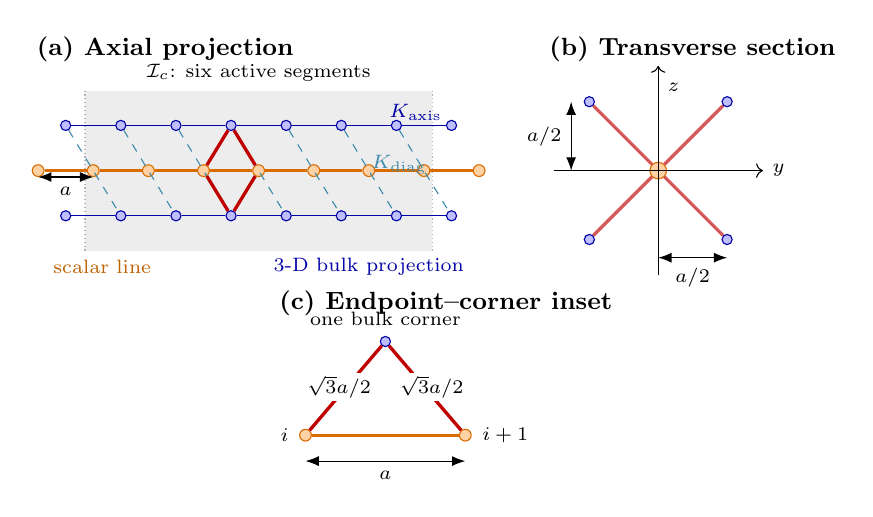
\begin{tikzpicture}[
    x=0.70cm,y=0.70cm,
    line/.style={draw=orange!85!black,very thick},
    linenode/.style={circle,draw=orange!85!black,fill=orange!35,inner sep=1.5pt},
    bulkbond/.style={draw=blue!65!black,thin},
    diagbond/.style={draw=cyan!65!black,thin,dashed},
    bulknode/.style={circle,draw=blue!65!black,fill=blue!25,inner sep=1.3pt},
    source/.style={draw=red!75!black,very thick},
    dim/.style={Latex-Latex,thin},
    lab/.style={font=\scriptsize},
    panel/.style={font=\bfseries\small}
]
% Panel A: axial projection
\begin{scope}[shift={(0,0)}]
  \node[panel,anchor=west] at (-0.2,2.20) {(a) Axial projection};
  \fill[gray!14] (0.85,-1.45) rectangle (7.15,1.45);
  \draw[gray!60,densely dotted] (0.85,-1.45) -- (0.85,1.45);
  \draw[gray!60,densely dotted] (7.15,-1.45) -- (7.15,1.45);
  \node[lab,anchor=south] at (4,1.45) {$\mathcal I_c$: six active segments};
  \foreach \i in {0,...,8}{\node[linenode] (q\i) at (\i,0) {};}
  \foreach \i in {0,...,7}{\draw[line] (q\i) -- (q\the\numexpr\i+1\relax);}
  \foreach \i in {0,...,7}{
    \node[bulknode] (bu\i) at (\i+0.5,0.82) {};
    \node[bulknode] (bd\i) at (\i+0.5,-0.82) {};
  }
  \foreach \i in {0,...,6}{
    \draw[bulkbond] (bu\i) -- (bu\the\numexpr\i+1\relax);
    \draw[bulkbond] (bd\i) -- (bd\the\numexpr\i+1\relax);
    \draw[diagbond] (bu\i) -- (bd\the\numexpr\i+1\relax);
  }
  \draw[source] (q3) -- (bu3);
  \draw[source] (q4) -- (bu3);
  \draw[source] (q3) -- (bd3);
  \draw[source] (q4) -- (bd3);
  \draw[dim] (q0.south) -- node[lab,below] {$a$} (q1.south);
  \node[lab,text=orange!75!black,anchor=west] at (0.1,-1.75) {scalar line};
  \node[lab,text=blue!65!black,anchor=east] at (7.9,-1.75) {3-D bulk projection};
  \node[lab,text=blue!65!black] at (6.85,1.06) {$K_{\rm axis}$};
  \node[lab,text=cyan!65!black] at (6.55,0.10) {$K_{\rm diag}$};
\end{scope}

% Panel B: transverse section
\begin{scope}[shift={(11.25,0)}]
  \node[panel,anchor=west] at (-2.15,2.20) {(b) Transverse section};
  \node[linenode,minimum size=6pt] (c0) at (0,0) {};
  \foreach \yy/\zz in {1/1,1/-1,-1/1,-1/-1}{
    \node[bulknode] (c\yy\zz) at (1.25*\yy,1.25*\zz) {};
    \draw[source,opacity=0.65] (c0) -- (c\yy\zz);
  }
  \draw[->,thin] (-1.9,0) -- (1.9,0) node[right,lab] {$y$};
  \draw[->,thin] (0,-1.9) -- (0,1.9) node[pos=0.90,right,lab] {$z$};
  \draw[dim] (0,-1.58) -- node[lab,below] {$a/2$} (1.25,-1.58);
  \draw[dim] (-1.58,0) -- node[lab,left] {$a/2$} (-1.58,1.25);
\end{scope}

% Panel C: 3-D endpoint/corner inset, centered below
\begin{scope}[shift={(6.3,-4.35)}]
  \node[panel,anchor=west] at (-2.1,1.95) {(c) Endpoint--corner inset};
  \node[linenode] (L) at (-1.45,-0.45) {};
  \node[linenode] (R) at (1.45,-0.45) {};
  \node[bulknode] (C) at (0,1.25) {};
  \draw[line] (L) -- (R);
  \draw[source] (L) -- (C);
  \draw[source] (R) -- (C);
  \draw[dim] (-1.45,-0.92) -- node[lab,below] {$a$} (1.45,-0.92);
  \node[lab,fill=white,inner sep=1pt] at (-0.84,0.42) {$\sqrt3a/2$};
  \node[lab,fill=white,inner sep=1pt] at (0.84,0.42) {$\sqrt3a/2$};
  \node[lab,anchor=east] at (-1.58,-0.45) {$i$};
  \node[lab,anchor=west] at (1.58,-0.45) {$i+1$};
  \node[lab,anchor=south] at (0,1.36) {one bulk corner};
\end{scope}
\end{tikzpicture}%
}
\caption{Reference geometry.  (a) Axial projection of the scalar line channel, one three-dimensional translated simple-cubic vector bulk, and the finite six-segment interaction slab.  The source-link motif shown on one segment is repeated on every active segment.  Representative bulk axial and face-diagonal bonds are keyed by $K_{\rm axis}$ and $K_{\rm diag}$.  (b) Transverse section at a segment midpoint.  The four corners are existing bulk nodes at $(s_y a/2,s_z a/2)$; each red radius is the projection of two distinct endpoint-to-corner links.  (c) Inset for one corner, showing endpoint separation $a$ and the two source-link rest lengths $\sqrt3a/2$.  Panel (a) is a projection of a single three-dimensional vector lattice, not a collection of independent planes.}
\label{fig:sectionII_geometry}
\end{figure*}

\subsection{Quadratic central-force origin}
\label{sec:s2-harmonic-origin}

For a generic bulk or source bond family $\alpha$, let
\begin{equation}
  \vd=r_{0,\alpha}\hat{\vd},
  \qquad
  V_\alpha'(r_{0,\alpha})=0,
  \qquad
  V_\alpha''(r_{0,\alpha})=\kappa_\alpha>0,
  \label{eq:s2-central-assumptions}
\end{equation}
where $V_\alpha\in C^3$ in a neighborhood of $r_{0,\alpha}$. For a relative displacement $\Delta\vu=\vu_j-\vu_i$ with $|\Delta\vu|\ll r_{0,\alpha}$,
\begin{align}
  |\vd+\Delta\vu|-r_{0,\alpha}
  &=\hat{\vd}\cdot\Delta\vu
    +\order\!\left(\frac{|\Delta\vu|^2}{r_{0,\alpha}}\right),
  \label{eq:s2-extension-expansion}\\
  V_\alpha(|\vd+\Delta\vu|)-V_\alpha(r_{0,\alpha})
  &=\frac{\kappa_\alpha}{2}
    (\hat{\vd}\cdot\Delta\vu)^2
    +\order(\Lambda_\alpha|\Delta\vu|^3),
  \label{eq:s2-energy-expansion}
\end{align}
with finite local coefficient $\Lambda_\alpha$. This is the usual harmonic central-force reduction~\cite{BornHuang1954,Maradudin1971}. We identify
\begin{equation}
  \kappa_{\rm ax}=K_{\rm axis},
  \qquad
  \kappa_{\rm fd}=K_{\rm diag},
  \qquad
  \kappa_{c,i}=g_i.
  \label{eq:s2-stiffness-map}
\end{equation}
The scalar line is an effective one-dimensional harmonic channel and need not be the restriction of the same microscopic pair potential. The retained quadratic expressions define the exact production model; Eqs.~\eqref{eq:s2-extension-expansion} and \eqref{eq:s2-energy-expansion} state one possible local mechanical origin.

No onsite pinning term or externally prescribed transverse force is present. Transverse restoring forces in the bulk arise from the intersite vector central-force network, particularly the face-diagonal family. An unstressed simple-cubic network containing only axis-aligned central springs would retain transverse floppy modes for propagation along a coordinate axis; the diagonal links remove that restricted no-shear pathology.

\subsection{Complete canonical Hamiltonian}
\label{sec:s2-hamiltonian}

Introduce canonical momenta
\begin{equation}
  p_i=m_q\dot q_i,
  \qquad
  \vp_{\bm r}=m_b\dot\vu_{\bm r}.
  \label{eq:s2-momenta}
\end{equation}
The Hamiltonian is
\begin{equation}
  H=H_q+H_b+H_c,
  \label{eq:s2-Htotal}
\end{equation}
where
\begin{equation}
  H_q
  =\sum_{i\in\mathbb Z}\frac{p_i^2}{2m_q}
  +\frac{K_q}{2}\sum_{i\in\mathbb Z}(q_{i+1}-q_i)^2,
  \label{eq:s2-Hq}
\end{equation}
\begin{align}
  H_b
  ={}&\sum_{\bm r\in\Lambdab}\frac{|\vp_{\bm r}|^2}{2m_b}
  \nonumber\\
  &+\frac12
  \sum_{\bm r\in\Lambdab}
  \sum_{\vd\in\mathcal D_{\rm ax}\cup\mathcal D_{\rm fd}}
  K_{\vd}
  \left[
  \hat{\vd}\cdot
  (\vu_{\bm r+\vd}-\vu_{\bm r})
  \right]^2,
  \label{eq:s2-Hb}
\end{align}
with $\Lambdab=\{\vR_{ijk}^{(b)}:i,j,k\in\mathbb Z\}$,
\begin{equation}
  K_{\vd}=
  \begin{cases}
    K_{\rm axis},&\vd\in\mathcal D_{\rm ax},\\
    K_{\rm diag},&\vd\in\mathcal D_{\rm fd},
  \end{cases}
  \qquad
  \hat{\vd}=\vd/|\vd|.
  \label{eq:s2-Kd}
\end{equation}
The positive representatives in Eqs.~\eqref{eq:s2-Dax} and \eqref{eq:s2-Dfd} count each undirected bulk bond once; the factor $1/2$ in Eq.~\eqref{eq:s2-Hb} is the physical spring-energy coefficient.

For one corner, write $\vu=\vu_{i,s_y,s_z}^{(c)}$ and define the equilibrium source-link directions
\begin{equation}
  \hat{\bm n}_L=\frac{(1,s_y,s_z)}{\sqrt3},
  \qquad
  \hat{\bm n}_R=\frac{(-1,s_y,s_z)}{\sqrt3}.
  \label{eq:s2-source-directions}
\end{equation}
The two physical links attached to that corner contribute
\begin{align}
  H_{c,i}^{(s_y,s_z)}
  ={}&\frac{g_i}{2}
  \left[
  \hat{\bm n}_L\cdot(\vu-q_i\ex)
  \right]^2
  \nonumber\\
  &+\frac{g_i}{2}
  \left[
  \hat{\bm n}_R\cdot(\vu-q_{i+1}\ex)
  \right]^2,
  \label{eq:s2-Hc-corner}
\end{align}
and the complete finite coupling Hamiltonian is
\begin{equation}
  H_c
  =\sum_{i\in\Ic}
   \sum_{s_y=\pm1}
   \sum_{s_z=\pm1}
   H_{c,i}^{(s_y,s_z)}.
  \label{eq:s2-Hc-total}
\end{equation}
With
\begin{equation}
  \bar q_i=\frac{q_i+q_{i+1}}{2},
  \qquad
  \Delta q_i=q_{i+1}-q_i,
  \label{eq:s2-qbar-delta}
\end{equation}
Eq.~\eqref{eq:s2-Hc-corner} reduces identically to
\begin{equation}
  H_{c,i}^{(s_y,s_z)}
  =\frac{g_i}{3}
  \left[
  (u_x-\bar q_i)^2
  +\left(
  s_yu_y+s_zu_z+\frac{\Delta q_i}{2}
  \right)^2
  \right].
  \label{eq:s2-Hc-reduced}
\end{equation}
This is an algebraic rotation of the two physical spring extensions, not a separately postulated interaction, a polarization decomposition, or a decomposition into the two lower bulk eigenbranches.

We assume
\begin{equation}
\begin{gathered}
  m_q,m_b,K_q,K_{\rm axis},K_{\rm diag}>0,\\
  g_i\ge0.
\end{gathered}
\label{eq:s2-positivity}
\end{equation}
The mass matrix is positive definite and the potential-energy stiffness matrix is real symmetric and positive semidefinite, hence $H\ge0$. Because $H$ has no explicit $\tau$ dependence, unforced Hamiltonian evolution conserves $H$; the model contains no gain, gyroscopic term, or velocity-dependent coupling. The underlying equations are therefore time-reversal invariant and reciprocal. The later scattering formulation verifies reciprocity with flux-normalized channels rather than relying only on this model-level statement.

The infinite sums in Eqs.~\eqref{eq:s2-Hq}--\eqref{eq:s2-Hc-total} are first understood on finite-energy configurations or finite volumes. Bloch and scattering states use per-cell or unit-flux normalization, followed by the standard infinite-volume scattering limit~\cite{Ong2018,Sadasivam2017,Khodavirdi2024}.

\subsection{Reference units, equilibrium, and nullspaces}
\label{sec:s2-units-nullspaces}

Take $a$, $m_b$, and $K_{\rm diag}$ as reference units. The dimensionless reference ratios are
\begin{equation}
  \frac{m_q}{m_b}=1,
  \qquad
  \frac{K_{\rm axis}}{K_{\rm diag}}=1,
  \qquad
  \frac{K_q}{K_{\rm diag}}=1.69,
  \label{eq:s2-ratios}
\end{equation}
with the six-segment source profile
\begin{equation}
  \frac{(g_{i_0},g_{i_0+1},\ldots,g_{i_0+5})}{K_{\rm diag}}
  =(0.1,0.2,0.2,0.2,0.2,0.1).
  \label{eq:s2-g-profile}
\end{equation}
The symmetric taper is a representative finite interaction profile, not a globally optimized design; its bounded comparison with four other six-segment profiles at the reference frequency and qT metric is reported in Sec.~\ref{sec:s9-robustness}. Dimensional units may be restored using
\begin{equation}
  [q]=[u]=a,
  \qquad
  [\tau]=\sqrt{m_b/K_{\rm diag}},
  \qquad
  [E]=K_{\rm diag}a^2.
  \label{eq:s2-units}
\end{equation}
Numerical frequencies below are quoted in units of $\sqrt{K_{\rm diag}/m_b}$; in particular, the displayed $\omega=1.2$ means $\omega\sqrt{m_b/K_{\rm diag}}=1.2$. Wavevectors retain inverse-length units and enter through dimensionless products such as $\vk a$.

At $q_i=0$ and $\vu_{ijk}=0$, every bond is at its rest length and all first derivatives of the potential vanish. The uncoupled line dispersion is
\begin{equation}
  \omega_q^2(k_x)
  =\frac{4K_q}{m_q}
   \sin^2\!\left(\frac{k_xa}{2}\right),
  \label{eq:s2-line-dispersion}
\end{equation}
with long-wave line speed
\begin{equation}
  c_q=\lim_{k_x\to0^+}\frac{\omega_q(k_x)}{k_x}
  =a\sqrt{\frac{K_q}{m_q}}.
  \label{eq:s2-line-speed}
\end{equation}
Thus the only first-Brillouin-zone zero is the uniform axial mode at $k_x=0$. For $K_{\rm axis},K_{\rm diag}>0$, the infinite bulk has three translational zero modes at $\vk=0$ and no nontrivial zero mode for $\vk\ne0$. This is the expected acoustic structure of a stable unpinned harmonic lattice~\cite{BornHuang1954,Maradudin1971}.

A free finite central-force cluster always contains rigid-body motions and may, for an arbitrary truncation, contain additional mechanisms. Under the stated free-boundary and included-bond convention, the tested $2\times2\times2$, $3\times2\times2$, $3\times3\times3$, and $4\times3\times3$ bulk fixtures each have exactly six rigid-body modes---three translations and three rotations---while the one- through four-segment combined line--bulk fixtures each have exactly two null modes. More generally, if the finite bulk framework is infinitesimally rigid, the scalar line is connected, and at least one complete positive four-corner/eight-link source motif is present, the combined kernel is exactly common axial translation plus rigid bulk rotation about the line. The Supplemental Material and validation archive provide the coordinate ordering, included-bond convention, tolerance, fixture records, and mutation controls. Exact finite-system counts remain boundary- and truncation-dependent. All scattering calculations are performed at finite frequency away from these zero modes.

The resulting passive finite-range quadratic model therefore contains a prepared scalar asymptotic channel, a stable three-dimensional vector bulk, and no prescribed transverse drive. The next section derives the forces generated by axial segment motion and establishes their reciprocal force, torque, and source-multipole structure.

\section{Local paired-link generation mechanism}
\label{sec:s3-mechanism}

The paired central-force links couple the axial average and the strain of each line segment to distinct corner-force patterns. Their derivation is standard harmonic lattice mechanics~\cite{BornHuang1954,Maradudin1971}; retaining the corner geometry identifies the relative signs and moments of those patterns. Force direction relative to the line is not a bulk-mode label: even in isotropic elasticity, an axial force can couple to a shear polarization for an off-axis propagation direction. We therefore retain both source patterns and later evaluate their projections onto the outgoing bulk modes. Let
\begin{align}
  \Cc&=\{(s_y,s_z):s_y,s_z=\pm1\},\\
  \vt_c&=s_y\ey+s_z\ez.
  \label{eq:s3-corners}
\end{align}
where $|\vt_c|=\sqrt2$.  For corner displacement $\vu_{ic}$ define
\begin{equation}
  \bar q_i=\frac{q_i+q_{i+1}}{2},
  \quad
  \Delta q_i=q_{i+1}-q_i,
  \quad
  S_{ic}=\vt_c\!\cdot\vu_{ic},
  \label{eq:s3-kinematic-defs}
\end{equation}
\begin{equation}
  A_{ic}=u_{ic,x}-\bar q_i,
  \qquad
  B_{ic}=S_{ic}+\frac{\Delta q_i}{2}.
  \label{eq:s3-AB}
\end{equation}
The exact per-corner coupling is
\begin{equation}
  H_{c,ic}=\frac{g_i}{3}\left(A_{ic}^{2}+B_{ic}^{2}\right).
  \label{eq:s3-Hcorner}
\end{equation}
The optional inverse-spacing dictionary
\begin{equation}
\begin{gathered}
  \epsilon_i=\Delta q_i/a,
  \qquad 1+\epsilon_i>0,\\
  n_{q,i}=[a+\Delta q_i]^{-1},
  \qquad n_{q,\mathrm{ref}}=a^{-1},\\
  \frac{n_{q,i}}{n_{q,\mathrm{ref}}}
  =(1+\epsilon_i)^{-1}
  =1-\epsilon_i+\order(\epsilon_i^2).
\end{gathered}
\label{eq:s3-density-dictionary}
\end{equation}
identifies positive $\Delta q_i$ with segment extension and negative $\Delta q_i$ with compression.  Equation~\eqref{eq:s3-density-dictionary} is only a kinematic interpretation; every force below follows from Eq.~\eqref{eq:s3-Hcorner}.

\subsection{Exact forces and line-driven source terms}
\label{sec:s3-forces}

Differentiating the same Hamiltonian with respect to the vector corner coordinate and the two scalar endpoint coordinates gives
\begin{align}
  \vF_{b,ic}
  &=-\frac{2g_i}{3}
  \left(A_{ic}\ex+B_{ic}\vt_c\right),
  \label{eq:s3-corner-force}\\
  Q_{i\leftarrow c}
  &=-\frac{\partial H_{c,ic}}{\partial q_i}
   =\frac{g_i}{3}(A_{ic}+B_{ic}),
  \label{eq:s3-left-generalized-force}\\
  Q_{i+1\leftarrow c}
  &=-\frac{\partial H_{c,ic}}{\partial q_{i+1}}
   =\frac{g_i}{3}(A_{ic}-B_{ic}).
  \label{eq:s3-right-generalized-force}
\end{align}
The endpoint quantities are axial generalized forces, not complete three-dimensional endpoint forces.  They obey the exact per-corner reciprocity identity
\begin{equation}
  \ex\!\cdot\vF_{b,ic}
  +Q_{i\leftarrow c}+Q_{i+1\leftarrow c}=0.
  \label{eq:s3-axial-reciprocity}
\end{equation}
Expanding Eq.~\eqref{eq:s3-corner-force} separates displacement-dependent restoring terms from the line-driven source components,
\begin{equation}
  \vF_{b,ic}
  =-\frac{2g_i}{3}
  \left(u_{ic,x}\ex+S_{ic}\vt_c\right)
  +\underbrace{\frac{2g_i}{3}\bar q_i\ex}_{\vF^{\rm src}_{X,ic}}
  +\underbrace{-\frac{g_i}{3}\Delta q_i\vt_c}_{\vF^{\rm src}_{R,ic}}.
  \label{eq:s3-source-split}
\end{equation}
At zero bulk displacement, $\vF^{\rm src}_{X,ic}+\vF^{\rm src}_{R,ic}$ is the full corner force.  Its transverse components are
\begin{equation}
  F_y=-\frac{g_i}{3}s_y\Delta q_i,
  \qquad
  F_z=-\frac{g_i}{3}s_z\Delta q_i.
  \label{eq:s3-initial-transverse-force}
\end{equation}
Thus segment extension drives all four corners toward the line, while compression reverses the pattern.  The response is a consequence of the autonomous spring energy; no transverse force is imposed independently.

\begin{figure*}[!t]
\centering
\resizebox{0.98\textwidth}{!}{%
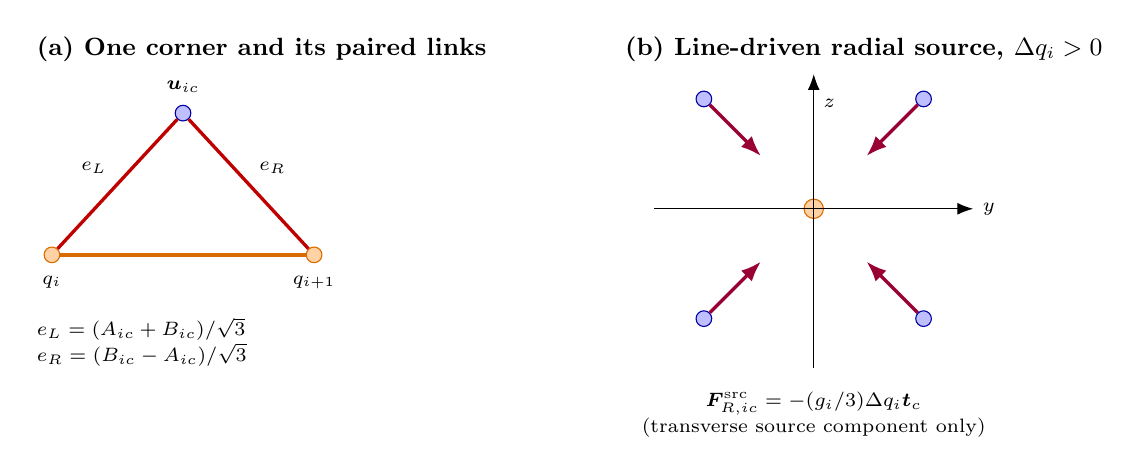
\begin{tikzpicture}[
  x=0.90cm,y=0.90cm,
  linenode/.style={circle,draw=orange!85!black,fill=orange!35,inner sep=2.0pt},
  bulknode/.style={circle,draw=blue!65!black,fill=blue!25,inner sep=2.0pt},
  spring/.style={draw=red!75!black,very thick},
  force/.style={-{Latex[length=2.6mm]},draw=purple!80!black,very thick},
  axis/.style={-{Latex[length=2.0mm]},thin},
  lab/.style={font=\scriptsize},
  panel/.style={font=\bfseries\small}
]
% Panel A
\begin{scope}[shift={(0,0)}]
  \node[panel,anchor=west] at (-2.2,2.25) {(a) One corner and its paired links};
  \node[linenode] (L) at (-1.85,-0.65) {};
  \node[linenode] (R) at (1.85,-0.65) {};
  \node[bulknode] (C) at (0,1.35) {};
  \draw[orange!85!black,very thick] (L)--(R);
  \draw[spring] (L)--node[lab,above left] {$e_L$}(C);
  \draw[spring] (R)--node[lab,above right] {$e_R$}(C);
  \node[lab,below=1pt of L] {$q_i$};
  \node[lab,below=1pt of R] {$q_{i+1}$};
  \node[lab,above=1pt of C] {$\vu_{ic}$};
  \node[lab,align=left,anchor=north west] at (-2.2,-1.40)
    {$e_L=(A_{ic}+B_{ic})/\sqrt3$\\$e_R=(B_{ic}-A_{ic})/\sqrt3$};
\end{scope}
% Panel B
\begin{scope}[shift={(8.9,0)}]
  \node[panel,anchor=west] at (-2.8,2.25) {(b) Line-driven radial source, $\Delta q_i>0$};
  \node[linenode,minimum size=7pt] (O) at (0,0) {};
  \foreach \yy/\zz in {1/1,1/-1,-1/1,-1/-1}{
    \node[bulknode] (B\yy\zz) at (1.55*\yy,1.55*\zz) {};
    \draw[force] (B\yy\zz) -- ($(B\yy\zz)!0.52!(O)$);
  }
  \draw[axis] (-2.25,0)--(2.25,0) node[right,lab] {$y$};
  \draw[axis] (0,-2.25)--(0,1.90) node[pos=0.90,right,lab] {$z$};
  \node[lab,align=center,anchor=north] at (0,-2.45)
    {$\vF^{\rm src}_{R,ic}=-(g_i/3)\Delta q_i\vt_c$\\(transverse source component only)};
\end{scope}
\end{tikzpicture}%
}
\caption{Local paired-link source. (a) One bulk corner is attached to both line endpoints by physical diagonal springs. The $X/R$ variables are exact linear combinations of their signed harmonic extensions. (b) For positive segment extension, the line-driven radial component points toward the line at all four corner sites $(s_y a/2,s_z a/2)$. The arrows show only $\vF^{\rm src}_{R,ic}$; the complete corner force also contains the axial source and displacement-dependent restoring terms. The exact resultant, torque, and first moment are given in Eqs.~\eqref{eq:s3-radial-balance}--\eqref{eq:s3-radial-dipole}.}
\label{fig:s3-mechanism}
\end{figure*}

\subsection{Balanced radial moment and finite-slab form factor}
\label{sec:s3-dipole-fourier}

With transverse corner radius
\begin{equation}
  \vrr_c=\frac{a}{2}\vt_c,
  \label{eq:s3-corner-radius}
\end{equation}
$\vF^{\rm src}_{R,ic}$ is collinear with $\vrr_c$.  Hence each radial source torque vanishes and the four-corner source satisfies
\begin{align}
  \sum_{c\in\Cc}\vF^{\rm src}_{R,ic}&=0,\\
  \sum_{c\in\Cc}\vrr_c\times\vF^{\rm src}_{R,ic}&=0.
  \label{eq:s3-radial-balance}
\end{align}
Using the elastodynamic moment convention
\begin{equation}
  M^R_{\alpha\beta}
  =\sum_{c\in\Cc}F^{\rm src}_{R,ic,\alpha}r_{c,\beta},
  \label{eq:s3-moment-definition}
\end{equation}
which is the standard first moment of a balanced force system~\cite{AkiRichards2002}, one obtains
\begin{equation}
  \bm M_i^R
  =-\frac{2g_i a\Delta q_i}{3}
  \operatorname{diag}(0,1,1).
  \label{eq:s3-radial-dipole}
\end{equation}
The source is therefore a symmetric transverse force dipole: contractile for $\Delta q_i>0$ and extensile for $\Delta q_i<0$.  Since $\operatorname{Tr}\bm M_i^R\ne0$, it is not purely deviatoric.

For the Fourier convention $e^{-i\vk\cdot\vrr}$, the transverse four-corner source factor is
\begin{equation}
  \widetilde{\vF}^{\rm src}_{R,i}(k_y,k_z)
  =\frac{4ig_i\Delta q_i}{3}
  \begin{pmatrix}
    0\\
    \sin(k_ya/2)\cos(k_za/2)\\
    \cos(k_ya/2)\sin(k_za/2)
  \end{pmatrix}.
  \label{eq:s3-local-fourier}
\end{equation}
For an arbitrary fixed-frequency dressed line state, write
\begin{align}
 q_i(\tau)&=\operatorname{Re}\!\left[Q_i^{\rm full}(\omega)e^{-i\omega\tau}\right],\\
 \Delta Q_i^{\rm full}(\omega)&=Q_{i+1}^{\rm full}(\omega)-Q_i^{\rm full}(\omega).
 \label{eq:s3-fixed-frequency-phasor}
\end{align}
The full finite-slab radial-source transform is
\begin{align}
  \widetilde{\vF}^{\rm slab}_{R}(\vk;\omega)
  &=\frac{4i}{3}\,\bm s_\perp(\vk)
  \sum_{i\in\Ic}g_i\Delta Q_i^{\rm full}(\omega)
  e^{-ik_x(i+1/2)a},\\
  \bm s_\perp(\vk)
  &=\begin{pmatrix}
    0\\
    \sin(k_ya/2)\cos(k_za/2)\\
    \cos(k_ya/2)\sin(k_za/2)
  \end{pmatrix}.
  \label{eq:s3-general-slab-source}
\end{align}
Thus the finite slab does not impose equality between the incident line wave number and the outgoing bulk component $k_x$. For the special pure line Bloch component $Q_i=Qe^{i\kappa ia}$, Eq.~\eqref{eq:s3-general-slab-source} factorizes through the aperture
\begin{equation}
  \mathcal A(\kappa-k_x)
  =\sum_{i\in\Ic}g_i
   e^{i(\kappa-k_x)(i+1/2)a}.
  \label{eq:s3-aperture}
\end{equation}
After removing the segment-midpoint phase and taking
$\rho^2=\kappa^2+k_y^2+k_z^2$ with $\rho a\ll1$,
\begin{equation}
 e^{-i\kappa(i+1/2)a}
 \widetilde{\vF}^{\rm src}_{R,i}
 =-\frac{2g_i a^2Q}{3}
  \begin{pmatrix}0\\ \kappa k_y\\ \kappa k_z\end{pmatrix}
 +\order(g_i|Q|a^4\rho^4).
 \label{eq:s3-long-wave-source}
\end{equation}
Force balance therefore removes the zero-wave-number radial monopole.  The form factor is generically nonzero at finite wave number but has symmetry-enforced nodal directions.

\subsection{\texorpdfstring{$X/R$}{X/R} work bookkeeping and centered scalar-sector consistency}
\label{sec:s3-XR-work}

The exact coupling separates algebraically into
\begin{equation}
  H_{X,ic}=\frac{g_i}{3}A_{ic}^2,
  \qquad
  H_{R,ic}=\frac{g_i}{3}B_{ic}^2.
  \label{eq:s3-XR-energies}
\end{equation}
If $e_L$ and $e_R$ are the two signed physical spring extensions in Fig.~\ref{fig:s3-mechanism}(a), then
\begin{equation}
  H_{X,ic}=\frac{g_i}{4}(e_L-e_R)^2,
  \qquad
  H_{R,ic}=\frac{g_i}{4}(e_L+e_R)^2.
  \label{eq:s3-XR-physical-springs}
\end{equation}
The corresponding complete coupling sectors are
\begin{equation}
\begin{aligned}
 H_X&=\sum_{i\in\Ic}\sum_{c\in\Cc}H_{X,ic},\\
 H_R&=\sum_{i\in\Ic}\sum_{c\in\Cc}H_{R,ic},\\
 H_c&=H_X+H_R.
\end{aligned}
 \label{eq:s3-XR-global}
\end{equation}
Thus $X$ is the axial-average component and $R$ is the segment-strain/radial component.  They are not the two lower bulk eigenbranches, not the $y/z$ spatial directions, and not two independently controllable polarizations.

Define the powers done by the coupling force on the bulk and line subsystems,
\begin{align}
  P_{b,X}^{ic}&=-\frac{2g_i}{3}A_{ic}\dot u_{ic,x},
  &P_{q,X}^{ic}&=\frac{2g_i}{3}A_{ic}\dot{\bar q}_i,
  \label{eq:s3-X-powers}\\
  P_{b,R}^{ic}&=-\frac{2g_i}{3}B_{ic}\dot S_{ic},
  &P_{q,R}^{ic}&=-\frac{g_i}{3}B_{ic}\dot{\Delta q}_i.
  \label{eq:s3-R-powers}
\end{align}
Because $g_i$ is time independent,
\begin{equation}
  \dot H_{X,ic}=-(P_{b,X}^{ic}+P_{q,X}^{ic}),
  \qquad
  \dot H_{R,ic}=-(P_{b,R}^{ic}+P_{q,R}^{ic}).
  \label{eq:s3-local-work}
\end{equation}
Global interface powers are obtained by summing over $i\in\Ic$ and $c\in\Cc$.  The power delivered to the line and bulk need not be instantaneously equal and opposite because the coupling energy can store energy.  Local work is exactly additive in $X$ and $R$; later quadratic field or flux observables may contain a cross term between same-full-state responses, but transmissions from separately ablated $X$-only and $R$-only Hamiltonians are not additive contribution fractions.

Finally, the scalar line is an effective axial channel rather than an unconstrained vector spine.  To test for hidden transverse constraint work, temporarily embed the two endpoints as vector coordinates.  On any centered $C_{4v}/A_1$-symmetric state of the form
\begin{equation}
  \vu_{ic}=U_{X,i}\ex+U_{R,i}\vt_c,
  \label{eq:s3-A1-state}
\end{equation}
where $U_{R,i}$ is the unnormalized coefficient of $\vt_c$, the quantities $A_{ic}$ and $B_{ic}$ are independent of $c$.  The transverse force on each embedded endpoint is therefore proportional to
\begin{equation}
  \sum_{c\in\Cc}\vt_c=0,
  \label{eq:s3-sign-sum}
\end{equation}
so
\begin{equation}
  \vF^{\rm emb}_{q_i,\perp}
  =\vF^{\rm emb}_{q_{i+1},\perp}=0.
  \label{eq:s3-embedded-reaction}
\end{equation}
Moreover, the complete $R$-channel bulk force is a corner-independent scalar times $\vt_c$, so its resultant vanishes and each term has zero torque about the segment midpoint. The $X$-channel bulk force is common and axial; its torque vanishes because $\sum_c\vrr_c=0$, while its axial resultant is cancelled by the two endpoint generalized forces through Eq.~\eqref{eq:s3-axial-reciprocity}. Together with Eq.~\eqref{eq:s3-radial-balance}, this gives complete force and torque closure on the centered $C_{4v}/A_1$ sector.  It does not establish off-symmetry vector-line dynamics.  The paired links have therefore mapped axial line displacement and segment strain into reciprocal bulk forces containing a balanced transverse dipole source.  This local result establishes the source structure, not radiation; the next section must determine whether the source populates outgoing quasi-transverse bulk modes using basis-invariant channel observables~\cite{Ong2018,Khodavirdi2024}.

\section{Three-dimensional bulk modes and exact source symmetry}
\label{sec:s4-bulk-symmetry}

Section~III establishes a reciprocal local source with a balanced transverse dipole component, but a local transverse force does not by itself establish a propagating transverse wave. We therefore determine the normal modes of the three-dimensional vector bulk, define the invariant quasi-transverse spectral cluster at the reference frequency, and identify the exact finite core symmetry sector containing the transversely centered scalar source. Flux normalization and outgoing power are deferred to Sec.~V.  The Bloch and symmetry constructions used here follow standard harmonic-lattice and point-group methods~\cite{BornHuang1954,Maradudin1971,Dresselhaus2008}.

\subsection{Bulk spectrum and invariant quasi-transverse cluster}
\label{sec:s4-bulk-spectrum}

For a bulk Bloch displacement
\begin{equation}
  \vu_{\vR}(\tau)
  =\operatorname{Re}\!\left[
    \ve_\lambda(\vk)
    e^{i(\vk\cdot\vR-\omega_\lambda\tau)}
  \right],
  \qquad
  \ve_\lambda^\dagger\ve_\mu=\delta_{\lambda\mu},
  \label{eq:s4-bloch-convention}
\end{equation}
the mass-normalized eigenproblem is
\begin{equation}
  D(\vk)\ve_\lambda(\vk)
  =\omega_\lambda^2(\vk)\ve_\lambda(\vk),
  \qquad
  -\frac{\pi}{a}\leq k_\alpha<\frac{\pi}{a}.
  \label{eq:s4-eigenproblem}
\end{equation}
Using one representative of every undirected axial and face-diagonal bond from Sec.~II gives
\begin{equation}
  D(\vk)
  =\frac{2}{m_b}
   \sum_{\bm d\in\mathcal D_{\rm ax}\cup\mathcal D_{\rm fd}}
   K_{\bm d}
   \left[1-\cos(\vk\cdot\bm d)\right]
   \hat{\bm d}\hat{\bm d}^{\mathsf T}.
  \label{eq:s4-dynamical-matrix}
\end{equation}
The factor follows from
$2-e^{i\vk\cdot\bm d}-e^{-i\vk\cdot\bm d}
 =2[1-\cos(\vk\cdot\bm d)]$.
For $K_{\rm axis},K_{\rm diag}>0$, every term in Eq.~\eqref{eq:s4-dynamical-matrix} is positive semidefinite.  At $\vk=0$, $D(0)=0$ and the bulk has the three uniform translations.  If $\vk\neq0$ in the first Brillouin zone, choose a coordinate $i$ with $k_i\neq0$.  The corresponding axial bond forces the $i$th component of any putative zero-polarization vector to vanish.  Every remaining component is then eliminated either by its own active axial bond or, when its wave-number component is zero, by a face diagonal containing directions $i$ and $j$.  Hence
\begin{equation}
  \ker D(\vk)=\{0\},
  \qquad \vk\neq0.
  \label{eq:s4-rigidity}
\end{equation}
The face-diagonal family is essential to this shear rigidity; axis-aligned central springs alone would retain transverse floppy modes along coordinate axes.

For the reference choice $K_{\rm axis}=K_{\rm diag}=K$, the operator-norm long-wave expansion is
\begin{equation}
  D(\vk)
  =\frac{Ka^2}{m_b}
   \left(|\vk|^2 I+2\vk\vk^{\mathsf T}\right)
   +\order\!\left(\frac{Ka^4}{m_b}|\vk|^4\right),
  \label{eq:s4-long-wave}
\end{equation}
so
\begin{equation}
  c_T=a\sqrt{K/m_b},
  \qquad
  c_L=\sqrt3\,c_T.
  \label{eq:s4-acoustic-speeds}
\end{equation}
The leading limit is isotropic, while the finite-spacing spectrum retains cubic anisotropy.

The scalar line has the exact dispersion
\begin{equation}
  \omega_q^2(\kappa)
  =\frac{4K_q}{m_q}
   \sin^2\!\left(\frac{\kappa a}{2}\right).
  \label{eq:s4-line-dispersion}
\end{equation}
At the reference frequency $\omega=1.2$, the positive right-moving root is
\begin{align}
  \kappa_q
  &=\frac{2}{a}\arcsin\!\left[
    \frac{\omega}{2}\sqrt{\frac{m_q}{K_q}}
  \right],\\
  \kappa_q a&=0.9594572754,\\
  \lambda_q&\equiv2\pi/\kappa_q,
  &\lambda_q/a=6.548686918.
  \label{eq:s4-line-carrier}
\end{align}
At fixed $k_x=\kappa_q$, the two lower branches each possess a regular $\omega=1.2$ level set in the transverse zone, whereas the upper-branch minimum over the full $(k_y,k_z)$ zone is
\begin{equation}
  \omega_{2,\min}(k_x=\kappa_q)=1.5988161301.
  \label{eq:s4-upper-threshold}
\end{equation}
Thus the two lower branches are kinematically available and the upper branch is unavailable only in the translation-invariant, conserved-$k_x$ comparison.  The actual six-segment slab does not conserve $k_x$ and therefore does not inherit that exclusion.

\begin{figure*}[!t]
  \centering
  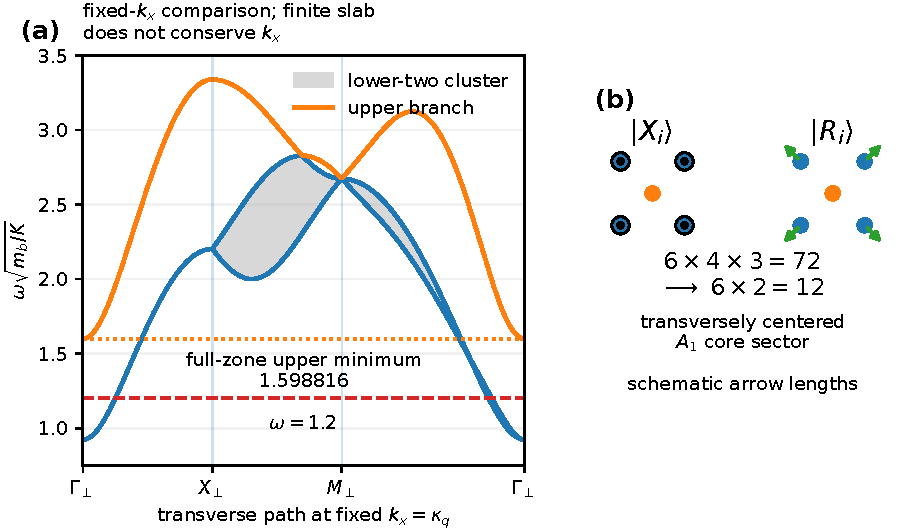
\includegraphics[width=0.98\textwidth]{figures/paper1_sectionIV_fig3_bulk_modes_symmetry_v2.pdf}
  \caption{Bulk modes and exact centered core symmetry.  (a) Exact bulk branches along
  $\Gamma_\perp(0,0)\rightarrow X_\perp(\pi/a,0)\rightarrow
  M_\perp(\pi/a,\pi/a)\rightarrow\Gamma_\perp(0,0)$ at fixed
  $k_x=\kappa_q$.  The horizontal line $\omega=1.2$ intersects both lower branches.  The quoted upper minimum $1.598816$ comes from a separate full two-dimensional transverse-zone optimization, not from assuming that the plotted path is exhaustive.  The upper branch is kinematically unavailable only when $k_x=\kappa_q$ is conserved; the finite slab does not conserve $k_x$.  (b) Normalized axial and radial $A_1$ patterns on one four-corner cross section.  Six segments give $6\times4\times3=72$ core coordinates but only $6\times2=12$ centered $A_1$ coordinates.  Arrow lengths are schematic symmetry patterns, not physical relative amplitudes or polarization controls.}
  \label{fig:s4-bulk-symmetry}
\end{figure*}

Order the branches by $\omega_0^2\leq\omega_1^2\leq\omega_2^2$ and define
\begin{equation}
  \Sigma_\lambda(\omega)
  =\{\vk\in\BZ:\omega_\lambda(\vk)=\omega\},
  \label{eq:s4-branch-shell}
\end{equation}
with an operating set $\Omega_{\rm op}\subset\BZ\setminus\{0\}$ on which
$\omega_2^2-\omega_1^2$ is bounded away from zero.  On this set,
\begin{equation}
  \PqL(\vk)=\ve_2\ve_2^\dagger,
  \qquad
  \PqT(\vk)=I-\PqL(\vk).
  \label{eq:s4-cluster-projectors}
\end{equation}
The lower eigenvectors may rotate inside a degenerate doublet, but the rank-two projector remains invariant.  A generic rotation of nondegenerate eigenvectors is not a new eigenbasis, and branch-dependent weights are invariant only when represented and transformed as full cluster operators.

The invariant wave-normal longitudinal leakage of the lower cluster is
\begin{equation}
  \ell_{\rm qT}^{(k)}(\vk)
  =\hat{\vk}^{\dagger}\PqT(\vk)\hat{\vk},
  \qquad \hat{\vk}=\vk/|\vk|.
  \label{eq:s4-cluster-leakage}
\end{equation}
Root-projected optimization on the exact reference shells gives the conservative bounds
\begin{align}
  \min_{\Sigma_0\cup\Sigma_1\cup\Sigma_2}
  (\omega_2^2-\omega_1^2)&>0.9390,\\
  \max_{\Sigma_0\cup\Sigma_1}
  \ell_{\rm qT}^{(k)}&<1.25\times10^{-3}.
  \label{eq:s4-gap-leakage-bounds}
\end{align}
\begin{equation}
  \min_{\Sigma_2}
  \hat{\vk}^{\dagger}\PqL(\vk)\hat{\vk}>0.99988.
  \label{eq:s4-upper-purity}
\end{equation}
The lower two-dimensional spectral cluster is therefore overwhelmingly quasi-transverse and remains well separated from the upper quasi-longitudinal branch at the operating frequency.  These are finite-frequency numerical bounds, not exact continuum identities.  Away from degeneracies and stationary points, $\bm v_{g,\lambda}=\nabla_{\vk}\omega_\lambda$; cubic anisotropy permits $\widehat{\bm v}_{g,\lambda}\neq\hat{\vk}$.  The Supplemental Material gives the shell definitions, conservative root-refined bounds, exact core-reduction residuals, and regular lower-shell witness coordinates and residuals. Full-precision extremizer coordinates, shell residuals, cluster gaps, projector diagnostics, and full/reduced response records are provided in the validation archive described in the Data Availability Statement.

\subsection{Exact centered core symmetry}
\label{sec:s4-core-symmetry}

For the centered scalar source, each four-corner section has two symmetry-allowed displacement patterns: a common axial displacement and a radial displacement. Six active sections therefore require twelve source-corner amplitudes. The projected Green response retains the surrounding infinite bulk; the reduction concerns the coordinates used to represent its response at the source corners.

Let $C_{4v}$ act about the line's $x$ axis, with displacements transforming as polar vectors.  Using the local active-segment labels $s=1,\ldots,N_c$ defined in Sec.~II, define the normalized core patterns
\begin{align}
  |X_s\rangle
  &=\frac12\sum_{c\in\Cc}|s,c,x\rangle,\\
  |R_s\rangle
  &=\frac{1}{2\sqrt2}
   \sum_{c=(s_y,s_z)}
   \left(s_y|s,c,y\rangle+s_z|s,c,z\rangle\right).
  \label{eq:s4-XR-basis}
\end{align}
They satisfy
$\langle X_s|X_t\rangle=\langle R_s|R_t\rangle=\delta_{st}$ and
$\langle X_s|R_t\rangle=0$.  For the six-segment core,
\begin{align}
  B&=\bigl(|X_1\rangle,|R_1\rangle,\ldots,
  |X_6\rangle,|R_6\rangle\bigr),\\
  B^\dagger B&=I_{12},
  &\PAone&=BB^\dagger.
  \label{eq:s4-core-basis}
\end{align}
This is the trivial-irrep projector on the finite core; equivalently it is obtained by the $C_{4v}$ group average~\cite{Dresselhaus2008}.

The distinction between symmetry and spatial support is essential.  The full bulk stiffness $K_b$ commutes with the full transverse group action and preserves the infinite-dimensional $A_1$ bulk sector, but it sends a displacement localized on the four source corners to neighboring sites outside the finite core.  Let $E_c$ embed the 72 core coordinates into the full bulk and define the core-projected retarded resolvent
\begin{equation}
  G_{cc}^R(\omega)
  =E_c^\dagger
   \left[K_b-m_b(\omega+i0^+)^2 I\right]^{-1}
   E_c.
  \label{eq:s4-core-resolvent}
\end{equation}
Let $V_c\in\mathbb R^{72\times7}$ be the full line-to-core source map and $U_c\in\mathbb R^{72\times72}$ the full local core stiffness induced by the source links.  Transverse centering gives
\begin{equation}
  \PAone V_c=V_c,
  \qquad
  [\PAone,U_c]=0,
  \qquad
  [\PAone,G_{cc}^R]=0.
  \label{eq:s4-exact-reduction-identities}
\end{equation}
Consequently,
\begin{equation}
  G_{cc}^R B
  =B\left(B^\dagger G_{cc}^R B\right),
  \label{eq:s4-reduced-resolvent}
\end{equation}
and the 72 source-corner coordinates admit an exact 12-coordinate $A_1$ core representation for the transversely centered scalar source.  The infinite bulk is retained through its projected Green matrix; Eq.~\eqref{eq:s4-reduced-resolvent} is not a truncation of the bulk itself.  Orthonormality, source and stiffness leakage, projected-resolvent leakage, and the full/reduced Green comparison close at approximately $10^{-15}$ or better under the declared regression norms.

There exists at least one regular, nondegenerate point on each lower branch shell at which the complete bare finite-slab $X+R$ line-driven source has nonzero resonant branch-projector overlap and nonzero group speed. The radial source component is also nonzero at the archived witnesses. This is a source-selection statement, not yet an outgoing-flux result: an unweighted geometric projection onto $\PqT$ would also include an off-shell lower polarization. The witness points and residuals are listed in the Supplemental Material; Sec.~V introduces the on-shell spectral measure and flux normalization required to convert branch overlap into physical branch power~\cite{Sadasivam2017,Ong2018,Khodavirdi2024}.

The vector bulk is therefore rigid away from the translational point, has an isolated quasi-transverse lower cluster at the operating frequency, and admits an exact centered 12-coordinate core representation while retaining the full infinite bulk response.  The next section constructs the corresponding retarded, flux-normalized scattering problem.

\section{Retarded, flux-normalized scattering formulation}
\label{sec:s5-scattering}

The calculation connects the source geometry to outgoing modal power in five steps. We first evaluate the isolated infinite bulk's response at the source corners in the centered basis, giving $g_0^R$. The complete paired-link Hessian supplies the core stiffness $U$, mixed block $V$, and line self-stiffness $K_{\rm self}$. Including $U$ in the projected bulk response gives the feedback $\Sigma_b^R$ on the line. Together with the two scalar-lead self-energies, this determines the seven-site response $G_D^R$. Finally, the work done by the physical source into each propagating cluster gives its outgoing power fraction. The infinite exterior is retained throughout through the projected response. This construction uses retarded Green-function, Caroli, and Fisher--Lee methods~\cite{BornHuang1954,Caroli1971,FisherLee1981,Sadasivam2017,Ong2018,Khodavirdi2024}.

We use
$x(\tau)=\operatorname{Re}[Xe^{-i\omega\tau}]$ and
$\ImH A=(A-A^\dagger)/(2i)$ throughout. On the real-frequency axis, a superscript $A$ denotes the advanced counterpart, equal to the Hermitian adjoint of the corresponding retarded object. Numerical quadratures and the detailed channel-normalization derivations are deferred to Sec.~VI and the Supplemental Material.

\subsection{Projected retarded problem}
\label{sec:s5-projected}

Let $\vq_D=(q_0,\ldots,q_6)^T$, with local active segment $s=1,\ldots,6$ joining $q_{s-1}$ to $q_s$, and let $|L\rangle=(1,0,\ldots,0)^T$, $|R\rangle=(0,\ldots,0,1)^T$.  The line device has $M_D=m_qI_7$ and $(K_D)_{ij}=2K_q\delta_{ij}-K_q(\delta_{i,j+1}+\delta_{i,j-1})$.  From the full core maps of Sec.~IV define the exact centered reductions
\begin{equation}
  V=B^\dagger V_c\in\mathbb R^{12\times7},
  \qquad
  U=B^\dagger U_cB\in\mathbb R^{12\times12}.
  \label{eq:s5-reduced-source-matrices}
\end{equation}
For the 12-coordinate core displacement amplitude $\vu_c$ in the orthonormal basis $B$, the real coupling stiffness is
\begin{align}
 H_{c,D}
 &=\tfrac12\vq_D^T K_{\rm self}\vq_D
 +\vu_c^T V\vq_D
 +\tfrac12\vu_c^T U\vu_c,\\
 K_{\rm self}&=K_{\rm self}^T,
 &U&=U^T.
 \label{eq:s5-block-stiffness}
\end{align}
where $K_{\rm self}\in\mathbb R^{7\times7}$ and the reduced $V,U$ are exact blocks of the paired-link Hessian.  The same real matrices act on complex monochromatic amplitudes.

The segment entries make this connection explicit. For local segment $s$, put $i=i_0+s-1$ and write $U_{X,s}=U_{X,i}$ and $U_{R,s}=U_{R,i}$ in the centered state of Eq.~\eqref{eq:s3-A1-state}. Its coefficients in the orthonormal patterns of Eq.~\eqref{eq:s4-XR-basis} are
\begin{align}
 \xi_s&=2U_{X,s}, & \zeta_s&=2\sqrt2 U_{R,s},\nonumber\\
 \vu_{s,c}&=\frac{\xi_s}{2}\ex
 +\frac{\zeta_s}{2\sqrt2}(s_y\ey+s_z\ez).
 \label{eq:s5-segment-coordinates}
\end{align}
This expression restricts the corner displacements to the centered $A_1$ sector. The coefficients retain displacement units, with reference scale $a$; the basis change introduces no mass weighting. In the order of $B$, $\vu_c=(\xi_1,\zeta_1,\ldots,\xi_6,\zeta_6)^T$.

Summing Eq.~\eqref{eq:s2-Hc-reduced} over the four corners gives
\begin{align}
 H_{c,s}^{(A_1)}=\frac{g_s}{3}\big[&
 (\xi_s-q_{s-1}-q_s)^2\nonumber\\[-2pt]
 &+(\sqrt2\zeta_s+q_s-q_{s-1})^2\big].
 \label{eq:s5-segment-energy}
\end{align}
For $\bm z_s=(\xi_s,\zeta_s)^T$ and $\bm Q_s=(q_{s-1},q_s)^T$, use the quadratic-form convention
\begin{align}
 H_{c,s}^{(A_1)}={}&\tfrac12\bm z_s^TU_s\bm z_s
 +\bm z_s^TV_s\bm Q_s\nonumber\\
 &+\tfrac12\bm Q_s^TK_{{\rm self},s}\bm Q_s.
 \label{eq:s5-segment-quadratic}
\end{align}
The blocks, all with stiffness units, are
\begin{align}
 U_s&=\frac{2g_s}{3}
 \begin{pmatrix}1&0\\0&2\end{pmatrix},\nonumber\\
 V_s&=\frac{2g_s}{3}
 \begin{pmatrix}-1&-1\\-\sqrt2&\sqrt2\end{pmatrix},\nonumber\\
 K_{{\rm self},s}&=\frac{4g_s}{3}I_2.
 \label{eq:s5-segment-hessian}
\end{align}
Assembling the segments adds their contributions at shared line endpoints. The ordinary line-spring matrix $K_D$ remains separate, with the lead-contact endpoint convention stated below. The numerical reference values use the units of Eq.~\eqref{eq:s2-units}.

Distinguish the infinite-bulk compliance, its 72-coordinate core projection, and its exact centered reduction.  Here $K_b$ is the Hessian of $H_b$ and $M_b=m_bI$ on the bulk displacement space:
\begin{align}
 \mathcal G_b^R&=[K_b-(\omega+i0^+)^2M_b]^{-1},\\
 G_{cc,0}^R&=E_c^\dagger\mathcal G_b^RE_c,
 &g_0^R&=B^\dagger G_{cc,0}^RB.
 \label{eq:s5-green-levels}
\end{align}
For Euclidean-normalized polarizations, let $c$ denote the 72 source-corner Cartesian coordinates embedded by $E_c$, and define
\begin{equation}
 [\bm\Phi_\lambda(\vk)]_A
 =\sum_{r\mu\in c}B_{r\mu,A}^*
 e_{\lambda\mu}(\vk)e^{i\vk\cdot\vR_r}.
 \label{eq:s5-form-factor}
\end{equation}
With dimensional $\vk$ and cell volume $a^3$,
\begin{align}
 g_0^R(\omega)
 &=\frac{a^3}{(2\pi)^3m_b}
 \sum_\lambda\int_{\BZ}d^3k\,
 \frac{\bm\Phi_\lambda\bm\Phi_\lambda^\dagger}
 {\omega_\lambda^2-(\omega+i0^+)^2},
 \label{eq:s5-bloch-resolvent}\\
 \ImH g_{0,C}^R
 &=\frac{\pi a^3}{(2\pi)^3m_b}
 \int_{\BZ}d^3k\sum_{\lambda\in C}
 \bm\Phi_\lambda\bm\Phi_\lambda^\dagger
 \delta(\omega_\lambda^2-\omega^2)\succeq0.
 \label{eq:s5-cluster-spectral}
\end{align}
where $C=\qT=\{0,1\}$ and $C=\qL=\{2\}$ on the operating interval where the upper branch is separated from the lower cluster.  At a regular simple-branch patch, Eq.~\eqref{eq:s5-cluster-spectral} becomes the co-area integral with denominator $|\nabla_{\vk}\omega_\lambda^2|=2\omega|\bm v_{g,\lambda}|$.  At an exact lower-doublet degeneracy, only the complete degenerate projector and cluster sum are canonical.  The modal cluster matrix is not a geometric wave-normal projection, and $\ImH g_0^R=\ImH g_{0,\qT}^R+\ImH g_{0,\qL}^R$.

Without assuming that $g_0^R$ is invertible,
\begin{align}
 g_c^R&=(I+g_0^RU)^{-1}g_0^R,
 &\Sigma_b^R&=-V^\dagger g_c^RV,
 \label{eq:s5-dressed-core}\\
 \Gamma_{b,C}
 &=2V^\dagger(I+g_0^AU)^{-1}
 \ImH g_{0,C}^R\\[-2pt]
 &\qquad\times(I+Ug_0^R)^{-1}V\succeq0,
 \label{eq:s5-cluster-linewidth}\\
 \Gamma_b&=\Gamma_{b,\qT}+\Gamma_{b,\qL}.
\end{align}
The complementary conventions $K-\omega^2M$ for the bulk and $\omega^2M-K-\Sigma$ for the device account for the minus sign in $\Sigma_b^R$ and yield $\Gamma_b=i(\Sigma_b^R-\Sigma_b^A)\succeq0$.  Constructing each cluster escape matrix from its positive on-shell measure avoids a post hoc basis split of the total projected Green matrix~\cite{Boumrar2025}.

For the right-moving scalar mode,
$\omega^2=(4K_q/m_q)\sin^2(\kappa a/2)$ with $0<\kappa a<\pi$.  In the declared seven-site contact partition,
\begin{align}
 \sigma_q^R&=-K_qe^{i\kappa a},
 &\gamma_q&=2K_q\sin(\kappa a),\\
 \Sigma_\alpha^R&=\sigma_q^R|\alpha\rangle\langle\alpha|,
 &\Gamma_\alpha&=\gamma_q|\alpha\rangle\langle\alpha|,
 \quad\alpha=L,R.
 \label{eq:s5-leads}
\end{align}
and
\begin{multline}
 G_D^R=\big[(\omega+i0^+)^2M_D-K_D-K_{\rm self}\\[-2pt]
 -\Sigma_L^R-\Sigma_R^R-\Sigma_b^R\big]^{-1}.
 \label{eq:deviceGreen}
\end{multline}
The endpoint diagonal convention in $K_D$ includes the springs crossing into the eliminated leads; the self-energies represent only their eliminated off-device response.

\subsection{Flux coefficients, current, reciprocity, and weak-coupling existence}
\label{sec:s5-flux}

Define the Caroli-normalized device response and dressed effective core source,
\begin{align}
 \vchi_D^{(L)}&=G_D^R\Gamma_L^{1/2}|L\rangle,\\
 \veta_c&=(I+Ug_0^R)^{-1}V\vchi_D^{(L)},\\
 \vf_c^{\rm eff}&=-\veta_c,
 &\vu_c^{(L)}&=-g_0^R\veta_c.
 \label{eq:s5-caroli-source}
\end{align}
The vector $\vchi_D^{(L)}$ is normalized for the Caroli trace, not to one unit of physical energy flux.  Under the stated phasor convention, a transparent scalar-chain amplitude $A$ carries $\overline P_q=(\omega\gamma_q/4)|A|^2$; hence
\begin{align}
 \vpsi_{D,{\rm phys}}^{(L)}&=2\vchi_D^{(L)}/\sqrt\omega,\\
 \vf_{c,{\rm phys}}^{\rm eff}&=-2\veta_c/\sqrt\omega.
 \label{eq:s5-physical-normalization}
\end{align}
carry unit incident energy flux.

The dimensionless outgoing fractions are
\begin{align}
 T_q&=\Tr[\Gamma_RG_D^R\Gamma_LG_D^A],
 \label{eq:s5-line-transmission}\\
 T_C&=\Tr[\Gamma_{b,C}G_D^R\Gamma_LG_D^A]
 =2\veta_c^\dagger\ImH g_{0,C}^R\veta_c\ge0.
 \label{eq:s5-cluster-transmission}
\end{align}
For a physical force $\vf$ and displacement $\vu=g_0^R\vf$,
\begin{align}
 \overline P
 &=\tfrac12\operatorname{Re}[\vf^\dagger(-i\omega\vu)]
 =\tfrac{\omega}{2}\vf^\dagger\ImH g_0^R\vf,\\
 \overline P_C
 &=\tfrac{\omega}{2}\vf^\dagger\ImH g_{0,C}^R\vf.
 \label{eq:s5-work-identity}
\end{align}
With $\vf=\vf_{c,{\rm phys}}^{\rm eff}$, $\overline P_C=T_C$.  Thus
$T_{\rm bulk}=T_{\qT}^{\rm modal}+T_{\qL}^{\rm modal}$ is the total fraction radiated into the complete infinite bulk, not a one-plane detector flux.  Away from internal lower-branch degeneracy, $T_{\qT}^{\rm modal}=T_0+T_1$; at exact degeneracy only the cluster object is canonical.

For one propagating scalar channel in each lead and the reciprocal phase convention,
\begin{align}
 r_L&=1-i\gamma_q[G_D^R]_{LL},
 &R_q&=|r_L|^2,\\
 R_q+T_q+T_{\rm bulk}&=1,
 \label{eq:s5-closure}\\
 T_{\rm bulk}&=T_{\qT}^{\rm modal}+T_{\qL}^{\rm modal}.
\end{align}
The sum follows from
$G_D^R-G_D^A=-iG_D^R(\Gamma_L+\Gamma_R+\Gamma_b)G_D^A$.

For each harmonic bond, half-bond site energy and directed current are~\cite{Hardy1963}
\begin{align}
 h_i&=\tfrac{m_i}{2}|\bm v_i|^2
 +\tfrac12\sum_{j\sim i}V_{ij},\\
 J_{i\to j}&=-\tfrac12(\bm v_i+\bm v_j)
 \cdot\bm F_{i\leftarrow j},\\
 \dot h_i+\sum_{j\sim i}J_{i\to j}&=0.
 \label{eq:bondcurrent}
\end{align}
For a simple Bloch displacement $\bm u_{\bm R}(\tau)=\operatorname{Re}[A\bm e_\lambda(\vk)e^{i(\vk\cdot\bm R-\omega_\lambda\tau)}]$,
$\overline{\bm{\mathcal J}}=\overline{\mathcal E}_{\lambda\vk}\bm v_{g,\lambda}$, where
$\overline{\bm{\mathcal J}}=\sum_{\bm d}\bm d\,\overline J_{0\to\bm d}$ and, for the Euclidean normalization $\ve_\lambda^\dagger\ve_\lambda=1$,
\begin{equation}
  \overline{\mathcal E}_{\lambda\vk}
  =\tfrac12m_b\omega^2|A|^2
\end{equation}
is the time-averaged total energy per primitive cell.  Local coherent currents can retain cross terms; asymptotic channels are orthogonal only under the declared flux bilinear or outgoing-packet limit, and an exactly degenerate lower sector is reported as an invariant cluster sum.

Because the mass and stiffness matrices are real symmetric and no active or gyroscopic term is present,
\begin{equation}
 S_{\alpha\beta}=S_{\widetilde\beta\,\widetilde\alpha},
 \label{eq:reciprocity}
\end{equation}
with tildes denoting time-reversed channels.  The representation $S=S^T$ requires compatible reciprocal phases.  Reciprocity alone does not require equal total bulk loss from opposite sides of an axially asymmetric profile.

Finally, scale $g_i\mapsto s g_i$ with $s\to0^+$, so that $U=sU_1$, $V=sV_1$, and $K_{\rm self}=sK_{{\rm self},1}$.  Let $\vchi_{D,0}^{(L)}$ denote the Caroli-normalized device response $\vchi_D^{(L)}$ evaluated at $s=0$.  On the regular operating region, away from lead thresholds, bulk stationary points, and dressed poles,
\begin{align}
 T_{\qT}^{\rm modal}(s,\omega)
 &=s^2\mathcal A_{\qT}(\omega)+\order(s^3),\\
 \mathcal A_{\qT}
 &=2\veta_{c,1}^\dagger\ImH g_{0,\qT}^R\veta_{c,1},\\
 \veta_{c,1}&=V_1\vchi_{D,0}^{(L)}.
 \label{eq:weak}
\end{align}
A regular simple-branch witness reported in the Supplemental Material and validation archive has nonzero shell gradient, nonzero spectral gaps, and $|\bm\Phi_\lambda^\dagger\veta_{c,1}|^2>0$; continuity therefore gives a shell patch of positive measure and $\mathcal A_{\qT}>0$.  Sufficiently weak positive coupling thus produces nonzero quasi-transverse transmission.  This local existence result does not determine the finite-coupling coefficient or a continuum limit.

The retarded formulation supplies nonnegative dimensionless line and bulk-cluster power fractions, an exact passivity sum rule, and a microscopic-current interpretation.  Section~VI evaluates two principal real-axis formulations and reports the reference partition and deterministic uncertainty.

\section{Frequency-domain evaluation and reference result}
\label{sec:s6-frequency}

Section~V defines the reflection and transmission coefficients as incident-energy-flux ratios and identifies $T_{\qT}^{\rm modal}$ as the invariant lower-two cluster output.  We now evaluate the principal-value and on-shell matrices at the reference point
\begin{equation}
 \omega=1.2,
 \qquad
 \frac{(g_1,\ldots,g_6)}{K_{\rm diag}}
 =(0.1,0.2,0.2,0.2,0.2,0.1).
 \label{eq:s6-reference-point}
\end{equation}
The point lies in a verified regular operating region, away from the scalar lead edges, shell stationary points, and dressed poles.  At this frequency, under the modal qT transmission metric and among the five tested six-segment profiles, the reference taper is not the maximizer; no global optimality claim is made.  All numerical ranges below are deterministic convergence or cross-formulation diagnostics rather than statistical uncertainties.

\subsection{Numerical formulations and reference partition}
\label{sec:s6-reference}

At the reference point, approximately $86.0\%$ of the incident power is transmitted along the line, $0.36\%$ is reflected, and $13.7\%$ enters the bulk. The lower acoustic cluster receives approximately $12.6\%$ of incident power and carries
\begin{equation}
 \frac{T_{\qT}^{\rm modal}}{T_{\rm bulk}}
 =0.9193555
 \label{eq:s6-generated-share}
\end{equation}
of the generated bulk power. Table~\ref{tab:s6-reference} gives the channel partition for the numerical formulations described below. The convergence diagnostics distinguish their central agreement from the remaining numerical sensitivities.

The controlling formulation combines a marching-surface quadrature of the real-axis bulk level sets on an $N=192$ periodic reciprocal grid~\cite{LorensenCline1987} with an order-$M=256$ Jackson--Chebyshev principal-value reconstruction averaged over two independently scrambled $2^{23}$-point Sobol samples~\cite{Weisse2006}. At degenerate grid nodes, the complete eigenspace projector is shared among its tied branches before interpolation. A separately implemented $N=192$ linear-tetrahedron calculation reconstructs the projected resolvent and modal powers from the same Hamiltonian and source geometry~\cite{Blochl1994}. It linearly interpolates each sorted eigenvalue, evaluates the matrix spectral weight at the tetrahedron centroid, and evaluates the analytic scalar resolvent with stable divided differences. The scalar integral uses $z=\omega^2+i10^{-10}$ to select the retarded logarithm branch. Both discretizations approximate the exact reciprocal-space integral. A retained generalized-Bloch calculation supplies representation-level corroboration~\cite{Ong2018}; its real part is extrapolated from finite $\eta$, and the value below is the low-pair linear-Richardson estimate.

\paragraph{AI-assisted research workflow.}
OpenAI ChatGPT, including GPT-5.6 Pro, assisted with portions of derivation checking, code generation and debugging, numerical-validation design and analysis, and literature organization. The author specified the physical model, assumptions, algorithms, and acceptance criteria; reviewed and corrected all incorporated output; and verified results against the stated equations, executable tests, machine-readable records, convergence checks, and separately implemented numerical formulations.

\begin{figure*}[t]
 \centering
 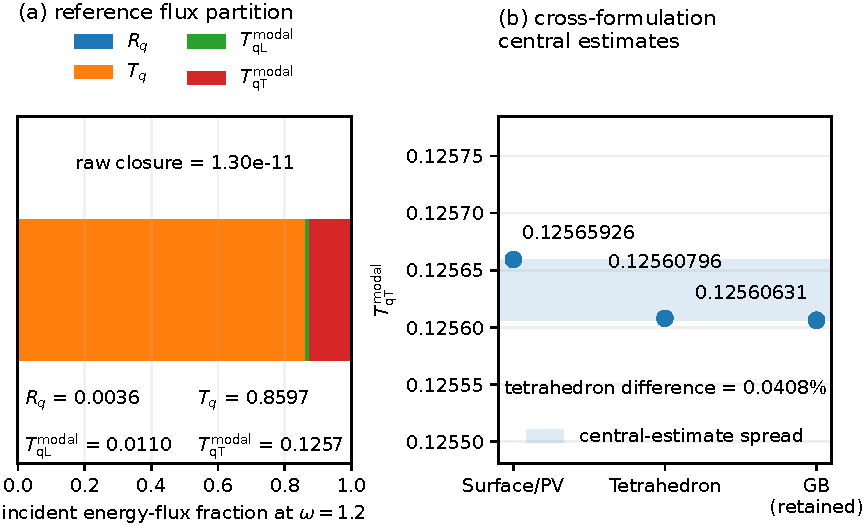
\includegraphics[width=0.98\textwidth]{figures/paper1_sectionVI_fig4_reference_partition_v2.pdf}
 \caption{Reference incident-power-normalized partition and cross-formulation comparison at $\omega=1.2$. (a) Fractions from the controlling $N=192$ surface/$M=256$ principal-value calculation, with closure evaluated before rounding. (b) Fresh surface and tetrahedron estimates and the retained generalized-Bloch extrapolation. The shaded band shows their central-estimate spread; convergence sensitivities are reported separately.}
 \label{fig:s6-reference}
\end{figure*}

\begin{table*}[t]
 \squeezetable
 \caption{Incident-power-normalized dimensionless partition. The listed values are central solver outputs rounded to the displayed digits so that method differences remain visible; their trailing digits are not certified physical precision.  The tetrahedron reflection is obtained from the independently evaluated reflection amplitude; a complement-defined value is used only as bookkeeping.  Full-precision outputs and separate convergence ladders are provided in the validation archive.}
 \label{tab:s6-reference}
 \begin{ruledtabular}
 \begin{tabular}{lccccc}
 Method & $R_q$ & $T_q$ & $T_{\rm bulk}$ & $T_{\qL}^{\rm modal}$ & $T_{\qT}^{\rm modal}$\\
 \hline
 Surface/PV & 0.0035721 & 0.8597460 & 0.1366819 & 0.0110226 & 0.1256593\\
 Linear tetrahedron & 0.0035701 & 0.8598070 & 0.1366229 & 0.0110150 & 0.1256080\\
 Generalized Bloch & 0.0035669 & 0.8598019 & 0.1366312 & 0.0110249 & 0.1256063\\
 \end{tabular}
 \end{ruledtabular}
\end{table*}

The central estimates span
\begin{equation}
 0.12560631\leq T_{\qT}^{\rm modal}\leq0.12565926,
 \label{eq:s6-central-range}
\end{equation}
with absolute range $5.295\times10^{-5}$; the tetrahedron value differs from the controlling value by $0.0408\%$. Separate surface, principal-value sampling/order, tetrahedron, and retained generalized-Bloch extrapolation diagnostics are given in the Supplemental Material. The central spread is not a complete numerical error bound. We quote the physical result as
\begin{equation}
 \boxed{T_{\qT}^{\rm modal}\simeq0.126.}
 \label{eq:s6-headline}
\end{equation}
For the controlling full-precision output,
\begin{equation}
 \left|R_q+T_q+T_{\qL}^{\rm modal}+T_{\qT}^{\rm modal}-1\right|
 =1.30\times10^{-11}.
 \label{eq:s6-closure}
\end{equation}
This is a stringent internal passivity and implementation check, not an independent validation of the Hamiltonian.

The wave-normal geometric diagnostic gives $T_{\perp k}^{\rm geom}=0.1256316$. Let $\theta$ be the angle between the group velocity and the line axis. Same-state angular decompositions on $N=80$ and $96$ grids reconstruct the total bulk power within $2.2\times10^{-4}$ relatively. Both have positive power in all eight octants, with minimum share about $1.3\%$, place about $94\%$ of the power at $\sin\theta>0.5$, and have weighted median $\sin\theta\simeq0.86$. These results support three-dimensional propagation over finite solid angle.

\subsection{Mechanism controls and elastic interpretation}
\label{sec:s6-controls}

The independently implemented $N=192$ tetrahedron calculation gives the positive surrogate-Hamiltonian controls in Table~\ref{tab:s6-ablation}. The $X$-only and $R$-only rows retain the same $H_q+H_b$ sectors and replace the physical coupling $H_c=H_X+H_R$ by $H_X$ or $H_R$, respectively. Every row is a separately dressed complete Hamiltonian, so the powers are not additive contribution fractions.

\begin{table}[t]
 \squeezetable
 \caption{Source-channel controls at $\omega=1.2$.  The full row is the physical paired-link Hamiltonian; the $X$-only and $R$-only rows are positive surrogate Hamiltonians.}
 \label{tab:s6-ablation}
 \begin{ruledtabular}
 \begin{tabular}{lccc}
 Hamiltonian & $T_{\rm bulk}$ & $T_{\qT}^{\rm modal}$ & $T_{\qT}^{\rm modal}/T_{\rm bulk}$\\
 \hline
 Full $X+R$ & 0.1366229 & 0.1256080 & 0.91938\\
 $X$ only & 0.1151728 & 0.1021905 & 0.88728\\
 $R$ only & 0.0024300 & 0.0022305 & 0.91791\\
 \end{tabular}
 \end{ruledtabular}
\end{table}

Fresh surface calculations of the $R$-only model give positive $\qT$ output at every tested frequency $\omega=0.8,1.0,1.2,1.4,1.7$, establishing that the radial/segment-strain channel is independently active. It is nevertheless subdominant at the reference point, and the reference coefficient belongs to the complete paired interaction. Define the coupling-sector interpolation and complete surrogate Hamiltonian by
\begin{equation}
\begin{aligned}
 H_c(\alpha)&=H_X+\alpha H_R,\\
 H(\alpha)&=H_q+H_b+H_c(\alpha),
 \qquad0\leq\alpha\leq1.
\end{aligned}
 \label{eq:s6-alpha-family}
\end{equation}
Thus $\alpha$ multiplies only the complete positive radial part of the coupling sector, while $H_q$ and $H_b$ remain fixed. Each $\alpha$ defines a separately dressed complete surrogate Hamiltonian; it is not a post-processing scale applied to a fixed source. $T_{\qT}^{\rm modal}$ rises monotonically on the tested 21-point grid from $0.1021905$ to $0.1256080$. This sampled trend is not an analytic monotonicity theorem.

For the physical full state, decompose the reduced source block as $V=V_X+V_R$ and use the same fully dressed line response in both terms:
\begin{equation}
\begin{aligned}
  \veta_\nu&=(I+Ug_0^R)^{-1}V_\nu\vchi_D^{(L)},
  &&\nu\in\{X,R\},\\
  \veta&=\veta_X+\veta_R.
\end{aligned}
  \label{eq:s6-same-state-source}
\end{equation}
With $Q_{\qT}=\ImH g_{0,\qT}^R$, define
\begin{equation}
\begin{aligned}
  T_{\nu\nu}&=2\veta_\nu^\dagger Q_{\qT}\veta_\nu,
  &&\nu\in\{X,R\},\\
  T_{XR}&=4\operatorname{Re}
  \left(\veta_X^\dagger Q_{\qT}\veta_R\right).
\end{aligned}
  \label{eq:s6-same-state-terms}
\end{equation}
The invariant modal-qT quadratic form then obeys the exact algebraic identity
\begin{equation}
 T_{\qT}^{\rm modal}=T_{XX}+T_{RR}+T_{XR}.
 \label{eq:s6-same-state-XR}
\end{equation}
with the controlling surface/PV values
\begin{equation}
 \begin{split}
 (T_{XX},T_{RR},T_{XR})\simeq{}&
 (0.10147813,0.00179177,\\
 &0.02238935).
 \end{split}
\end{equation}
The terms are the $X$ self, $R$ self, and $X$--$R$ cross terms. In this full state, the positive cross term is approximately $17.8\%$ of the displayed total modal-qT power. The independent $N=192$ tetrahedron cross term differs by $0.026\%$. These are algebraic terms in one quadratic form, not separately conserved energies.

The redressed controls answer a different question. In the tetrahedron calculation, replacing $H_X$ by the full $H_X+H_R$ raises $T_{\qT}^{\rm modal}$ from $0.1021905$ to $0.1256080$, a change of about $2.34$ percentage points of incident power. That difference includes the changed scattering state and is not the same-state cross term. The small $R$-only coefficient therefore does not measure the radial sector's effect on the combined response.

For interpretation, a time-harmonic axial point force in an unbounded isotropic elastic medium radiates shear and compressional power in the ratio~\cite{Achenbach1973,Graff1975}
\begin{equation}
 \frac{P_S}{P_P}=2\left(\frac{c_L}{c_T}\right)^3.
 \label{eq:s6-point-force}
\end{equation}
With $c_L/c_T=\sqrt3$, the shear share is $0.91222145$.  An undressed first-Born isotropic-continuum source benchmark using the finite six-segment $X$ and $R$ form factors gives shear fractions $0.87495206$ ($X$), $0.91771932$ ($R$), and $0.91914369$ (coherent $X+R$), close to the lattice generated-bulk share $0.91935554$. Finite axial and radial line-source radiation provides a related conventional source-class comparison~\cite{Aldridge1998}. The continuum S fractions and the lattice modal-qT fraction are analogous generated-bulk shares but are not identical observables. This benchmark provides a conventional elastodynamic compatibility scale for the generated-bulk shear share. It does not predict the absolute line-to-bulk transmission or the dressed finite-slab scattering state.

The complete sampled $\alpha$ scan and the first-Born/lattice share comparison are provided in the Supplemental Material. Their machine-readable values and producer code are provided in the validation archive.


The frequency-domain calculations therefore establish a nonzero incident-power-normalized modal-qT transmission fraction of approximately $0.126$, with the lower cluster carrying approximately $91.9\%$ of generated bulk power.  The radial source is independently active but does not dominate the reference coefficient, and the large lower-cluster share is compatible with ordinary elastic radiation.  Section~VII tests the same Hamiltonian using a real right-moving packet and exactly zero initial bulk displacement and velocity.

\section{Real-time packet corroboration}
\label{sec:s7-direct}

Section~VI determines the asymptotic monochromatic coefficient, whereas a real packet samples a finite frequency interval.  We therefore evolve the original finite real-space Hamiltonian directly, without eliminating either subsystem and without damping or an external drive after preparation.  A symmetric Verlet scheme~\cite{Verlet1967} advances the scalar line and the complete vector bulk.  The packet carrier is fixed at the reference operating frequency.  This calculation is an independent numerical solution of the same Hamiltonian, not an independent physical model and not an experimental validation.

\subsection{Packet, interface current, and interval selection}
\label{sec:s7-packet}

The initial line displacement is
\begin{align}
 q_i(0)
 &=A e^{-(ia-x_c)^2/(2\sigma_x^2)}
 \cos[\kappa_0(ia-x_c)],\\
 (A,x_c,\sigma_x)&=(0.002a,18a,7a).
 \label{eq:s7-packet}
\end{align}
where $\omega_0=1.2$ and $\kappa_0a=0.9594572754$.  For the finite-grid line diagnostics, let $N_{\rm line}$ be the number of line sites in the periodic diagnostic representation and use the unnormalized forward transform
\begin{equation}
 \widehat q(k)=\sum_{j=0}^{N_{\rm line}-1}q_j e^{-ikja},
 \qquad
 q_j=\frac{1}{N_{\rm line}}\sum_k\widehat q(k)e^{ikja},
 \label{eq:s7-line-dft}
\end{equation}
with the same convention for $\widehat{\dot q}$. Define the scalar-line group velocity $v_{g,q}(k)=\partial\omega_q(k)/\partial k$. Its velocity is constructed from the exact uncoupled-line dispersion,
\begin{equation}
 \widehat{\dot q}(k,0)
 =-i\,\operatorname{sgn}[v_{g,q}(k)]\,
 \omega_q(k)\widehat q(k,0),
 \label{eq:s7-packet-velocity}
\end{equation}
with the zero and Nyquist components treated separately.  Under the finite-grid periodic Parseval decomposition, $0.9999997423$ of the periodic spectral energy is right moving; the remaining $2.58\times10^{-7}$ is the stationary Nyquist component. That periodic spectral energy differs from the open-line $E_0=H_q(0)$ by $9.18\times10^{-9}$ relatively because the periodic representation contains a closing bond absent from the open production line.  Because Eq.~\eqref{eq:s7-packet-velocity} is imposed spectrally while the production line is finite and open, translated long-line controls were also performed. In each line, cumulative incident flux is evaluated through the bond immediately preceding the coupling slab: bond $59$ in the 120-site production line and the correspondingly translated bond in each longer control. Relative to the converged 160-site control, the production line changes cumulative incident flux by $2.35\times10^{-4}$ at $\tau=52$, $2.22\times10^{-4}$ at $\tau=55$, and $2.20\times10^{-4}$ at $\tau=55.4$; the 160-, 200-, and 240-site controls agree within $6.8\times10^{-14}$ relatively.

Every bulk coordinate starts from
\begin{equation}
 \bm u_{\bm r}(0)=\dot{\bm u}_{\bm r}(0)=0.
 \label{eq:s7-unexcited-bulk}
\end{equation}
The finite packet leaves only $E_c(0)/E_0=2.05\times10^{-18}$ in the source links, where $E_0=H_q(0)$ is the prepared line energy.  Its energy-weighted $1\%$--$99\%$ frequency interval is $0.932\lesssim\omega\lesssim1.473$, so the later comparison uses a packet average rather than the carrier coefficient.  The production truncation uses a 120-site scalar line and a $120\times56\times56$ vector bulk with open (free) boundaries in every finite direction: bonds that would leave either domain are omitted, and no wraparound bonds are present. The six-segment coupling slab occupies line segments $60$--$65$, and the timestep is $\Delta\tau=0.04$.

For every source link counted once, the exact harmonic bond current is~\cite{Hardy1963}
\begin{align}
 J_{i\to j}
 &=-\tfrac12(\bm v_i+\bm v_j)
 \cdot\bm F_{i\leftarrow j},\\
 \bm v_i&=\dot q_i\hat{\bm x}
 \quad\text{on a line endpoint}.
 \label{eq:s7-current}
\end{align}
With half of each coupling-link energy assigned to each subsystem,
\begin{equation}
 \int_0^\tau J_{q\to b}(\tau')\,d\tau'
 =\Delta E_b(\tau)+\frac12\Delta E_c(\tau).
 \label{eq:s7-current-balance}
\end{equation}
Integrating the interface current from $\tau=0$ at every $\Delta\tau=0.04$ velocity-Verlet level with the composite trapezoidal rule, and comparing at the cadence-$0.2$ times in the accepted interval, gives a maximum assigned-gain-relative residual of $0.0297\%$; the exact statistic is defined in the Supplemental Material.

The final selector uses only direct-dynamics quantities over $48\le\tau\le57$ and is evaluated at a commensurate cadence $0.2$.  Here $E_b^{\rm open}$ is the direct open-box bulk Hamiltonian energy, $E_{\rm bulk}^{\rm per}$ is the total energy of the periodic Fourier embedding of the same snapshot, and $f_{\rm shell}^{\rm kin}$ is the fraction of total bulk kinetic energy in the two-cell transverse ($y,z$) boundary strips.  It requires a minimum accepted duration $2.0$ and selects the longest accepted interval, with the earliest start as tie breaker.  Its predicates are
\begin{gather}
 E_c/E_0\le2.5\times10^{-3},\qquad
 |J_{q\to b}|/E_0\le5.0\times10^{-4},\\
 f_{\rm shell}^{\rm kin}\le2.0\times10^{-3},\qquad
 \delta_{\rm per/open}\le2.5\times10^{-3},\\
 |H(\tau)-H(0)|/H(0)\le10^{-5}.
 \label{eq:s7-selector-a}
\end{gather}
Here
\begin{equation}
 \delta_{\rm per/open}
 =\frac{|E_{\rm bulk}^{\rm per}-E_b^{\rm open}|}{E_b^{\rm open}}.
 \label{eq:s7-selector-b}
\end{equation}
No frequency-domain coefficient enters these predicates.  The resulting coefficient-blind reporting interval is
\begin{equation}
 \boxed{52.8\le\tau\le55.4.}
 \label{eq:s7-window}
\end{equation}
The interval-selection predicate in Eq.~\eqref{eq:s7-selector-a} uses the transverse kinetic shell.  An independent post-selection recertification that assigns kinetic energy and half of each incident bulk-bond energy to every node gives a maximum unique-union six-face shell fraction $1.858\times10^{-3}$ over Eq.~\eqref{eq:s7-window}.

\begin{figure*}[t]
 \centering
 \begin{minipage}[t]{0.48\textwidth}\centering
  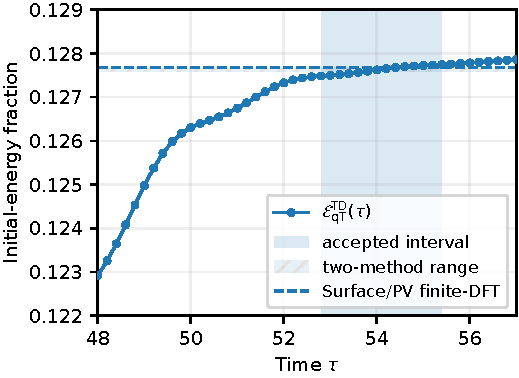
\includegraphics[width=\linewidth]{figures/paper1_sectionVII_fig6a_qT_window_v2.pdf}\\[-2pt]\small (a)
 \end{minipage}\hfill
 \begin{minipage}[t]{0.48\textwidth}\centering
  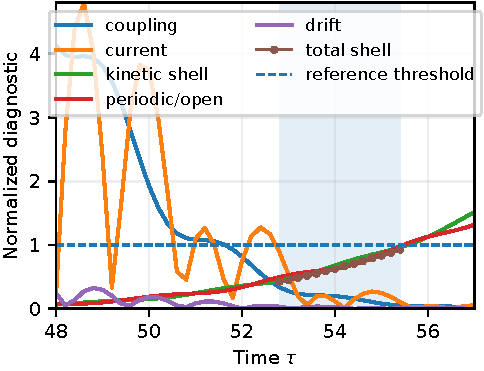
\includegraphics[width=\linewidth]{figures/paper1_sectionVII_fig6b_selector_controls_v2.pdf}\\[-2pt]\small (b)
 \end{minipage}
 \caption{Real-time packet calculation with a coefficient-blind reporting window. Time $\tau$ is expressed in units of $\sqrt{m_b/K_{\rm diag}}$. (a) Finite-time lower-cluster energy fraction and the accepted interval. The surface $N=160$ finite-DFT prediction and the range between it and the tetrahedron $N=128$ prediction are overlaid after the interval is selected. (b) Time-domain selector diagnostics divided by their declared thresholds. The total-shell curve is an independent post-selection recertification and was not used to select the interval.}
 \label{fig:s7-dynamics}
\end{figure*}

\subsection{Invariant lower-cluster energy and numerical corroboration}
\label{sec:s7-result}

A periodic Fourier embedding of each finite snapshot provides the global branch-content diagnostic.  Let $N=N_xN_yN_z$ be the number of bulk cells in that periodic embedding. For the integer cell indices $\bm n$ of the diagnostic array, we use
\begin{equation}
 \widehat{\bm u}(\vk)=\sum_{\bm n}\bm u_{\bm n}e^{-i\vk\cdot a\bm n},
 \qquad
 \bm u_{\bm n}=\frac{1}{N}\sum_{\vk}\widehat{\bm u}(\vk)e^{i\vk\cdot a\bm n},
 \label{eq:s7-bulk-dft}
\end{equation}
with the same convention for $\widehat{\dot{\bm u}}$. Because $D(\vk)$ is mass normalized, the exact energy of this periodic embedding is
\begin{equation}
 E_{\rm bulk}^{\rm per}
 =\frac{m_b}{2N}\sum_{\vk}
 \left[
  \widehat{\dot{\bm u}}^{\dagger}\widehat{\dot{\bm u}}
  +\widehat{\bm u}^{\dagger}D(\vk)\widehat{\bm u}
 \right].
 \label{eq:s7-periodic-total-energy}
\end{equation}
Away from exact upper--middle degeneracy, the upper-mode energy is~\cite{BornHuang1954}
\begin{align}
 E_{\qL}^{\rm per}
 &=\frac{m_b}{2N}\sum_{\bm k}
 \left[
 |\bm e_2^\dagger\widehat{\dot{\bm u}}|^2
 +\omega_2^2|\bm e_2^\dagger\widehat{\bm u}|^2
 \right],\\
 E_{\qT}^{\rm per}
 &=E_{\rm bulk}^{\rm per}-E_{\qL}^{\rm per}.
 \label{eq:s7-modal-energy}
\end{align}
At exact upper--middle doublets and threefold degeneracies, the complete-subspace energy-coherence matrix defined in the Supplemental Material is retained on the complete degenerate eigenspace and its eigenvalues bound the one-dimensional $\qL$ allocation.  Over Eq.~\eqref{eq:s7-window}, the resulting time-averaged $\qT$ ambiguity is only $9.52\times10^{-10}$ in units of $E_0$.  The exact-degeneracy allocation bounds and their midpoint are basis invariant, but this modal allocation is spatially nonlocal; it is not a unique local $\qT/\qL$ current.

For the stored cadence $h=0.2$, define $\mathcal E_{\qT}^{\rm TD}(\tau)=E_{\qT}^{\rm per}(\tau)/E_0$ and let $\overline{\mathcal E}_{\qT,h}^{\rm TD}$ be its composite-trapezoidal average over $[\tau_a,\tau_b]$. The finite sum and the full-precision allocation bounds are given in the Supplemental Material. The physical result is
\begin{equation}
 \overline{\mathcal E}_{\qT,h}^{\rm TD}\simeq0.1276.
 \label{eq:s7-direct-result}
\end{equation}
This is a stored-cadence window average, not an exact continuous-time integral. The degeneracy-allocation interval described above excludes quadrature and other numerical errors. The sampled instantaneous range is $0.1274833$--$0.1277449$. The corresponding qL and periodic-bulk averages are $0.0113021$ and $0.1389284$, so the lower cluster contains approximately $91.9\%$ of the periodic modal bulk energy. These are finite-time stored-energy fractions, not measurements of an asymptotic local branch flux.

For the declared 120-point DFT preparation, the stationary spectral comparison is
\begin{equation}
 T_C^{\rm packet}
 =\frac{\sum_k W(k)T_C[\omega_q(k)]}{\sum_k W(k)}.
 \label{eq:s7-packet-average}
\end{equation}
The fresh calculation evaluates all fourteen distinct DFT frequencies in $\mathcal K=\{k:0.8\le\omega_q(k)\le1.6\}$, with packet-energy coverage $c_{\mathcal K}=\sum_{k\in\mathcal K}W(k)/\sum_kW(k)=0.9996834928$. Its in-band contribution is normalized by the full packet energy: $S_{C,\mathcal K}=\sum_{k\in\mathcal K}W(k)T_C[\omega_q(k)]/\sum_kW(k)$. Passivity therefore gives
\begin{equation}
 S_{C,\mathcal K}\le T_C^{\rm packet}
 \le S_{C,\mathcal K}+1-c_{\mathcal K}.
 \label{eq:s7-packet-tail-bound}
\end{equation}
The surface/$M=256$ PV calculation at $N=160$ gives $S_{\qT,\mathcal K}=0.1276730$, whose prediction-normalized difference from the unchanged direct window average is $0.0365\%$. The independent $N=128$ tetrahedron result is $0.1275947$, a $0.0614\%$ difference between methods. Both use direct evaluations at every weighted frequency, so the finite-DFT central sums require no interpolation. Complete mesh-refinement and incoming-spectrum comparisons are reported separately in the Supplemental Material.

Equation~\eqref{eq:s7-packet-tail-bound} gives the conditional full-grid interval $[0.1276730,0.1279895]$. The direct average lies slightly below its lower endpoint: the interval bounds the omitted spectral weight, not integration or finite-time estimator error. The finite-box, time-step and cadence comparisons below address separate numerical sensitivities.

The cadence-$0.4$ selector returns $52.8\leq\tau\leq55.2$; its selected-window qT average differs by $0.00749\%$ from the cadence-$0.2$ result on $52.8\leq\tau\leq55.4$. On their common interval $52.8\leq\tau\leq55.2$, the cadence-only trapezoidal difference is $8.16\times10^{-5}\%$.  At exactly common times, the $\Delta\tau=0.03,0.04,0.05$ averages span $0.00160\%$.  Over all 66 time levels (65 velocity-Verlet advances) in the selected interval, $\max |H(\tau)-H(0)|/H(0)=3.54\times10^{-7}$.  On the fixed final interval $52.8\leq\tau\leq55.4$, enlarging the transverse box from $56\times56$ to $64\times64$ changes the invariant qT average by $0.04398\%$ and the periodic total by $0.10498\%$, while qL changes by $0.7938\%$ and therefore receives no stronger precision claim. The selected-window time averages of the cumulative current-transfer fraction $E_0^{-1}\int_0^\tau J_{q\to b}(\tau')\,d\tau'$ and the open bulk-energy fraction $E_b^{\rm open}/E_0$ change by less than $4.4\times10^{-8}$ relatively.

The real-time calculation therefore corroborates two claims independently of the retarded solver: energy is transferred from the prepared line into an initially unexcited bulk, and the generated bulk energy predominantly occupies the invariant lower-two acoustic cluster.  It does not define a remote local $\qT$ flux or a detector-plane complex field.

\section{Robustness, scaling, and model scope}
\label{sec:s9-robustness}

Weak-coupling, continuity, and numerical calculations describe complementary aspects of robustness. First, for a fixed profile scaled by $s$, Sec.~V proves
\begin{equation}
T_{\qT}^{\rm modal}(s,\omega)
=s^2\mathcal A_{\qT}(\omega)+\order(s^3),
\qquad \mathcal A_{\qT}(\omega)>0,
\label{eq:s9-weak-neighborhood}
\end{equation}
under the stated regular-shell, threshold, and pole hypotheses. Hence $T_{\qT}^{\rm modal}>0$ for all sufficiently small positive $s$. This perturbative statement is centered at $s=0$; it does not by itself establish a neighborhood of the finite reference scale.

Second, consider the continuous parameters of the fixed-topology model, with the graph, slab support, and bond inventory held fixed. Away from lead thresholds, stationary shell points, closure of the upper/lower cluster gap, and dressed poles, the self-energies, separated cluster measure, dressed device inverse, and Caroli coefficient are continuous. The reference coefficient is strictly positive and the verified regularity margins are nonzero. Continuity therefore implies an unquantified open neighborhood of the finite reference point in this fixed-topology continuous-parameter space on which $T_{\qT}^{\rm modal}>0$. No numerical radius is claimed, and discrete changes such as slab length or graph topology are not coordinates of this neighborhood.

Third, the declared one-factor calculations provide finite sampled evidence. They comprise 49 frequencies $0.6\leq\omega\leq1.8$, ten positive coupling scales $0.05\leq s\leq2$, six slab lengths $N_c=2,3,4,6,8,10$, five six-segment profiles, ten line long-wave speeds $0.65\leq c_q\leq2.0$, and five stiffness ratios $0.75\leq K_{\rm diag}/K_{\rm axis}\leq1.25$. Modal qT power is positive in all 85 sampled positive-coupling configurations, with maximum flux-closure residual $3.97\times10^{-11}$ and maximum modal-sum residual $8.33\times10^{-17}$. The frequency family spans $0.1049\leq T_{\qT}^{\rm modal}\leq0.2177$. These are sampled one-factor results, not a multivariate or continuous-domain theorem. The Supplemental Material~\cite{SupplementalMaterial} gives the family definitions and summaries; complete row-level values, numerical encodings, regularity metadata, and producer code are provided in the validation archive.

The overall-coupling family illustrates how the partition changes at fixed frequency and profile shape. At $\omega=1.2$, scaling the complete reference coupling as $g_i\mapsto s g_i$ gives $T_{\qT}^{\rm modal}\simeq0.1257,0.3089,0.5222$ at $s=1,1.5,2$, respectively, in the surface calculation with grid $N=80$ and PV order $M=256$. At $s=2$, the incident-power fractions $(R_q,T_q,T_{\qT}^{\rm modal},T_{\qL}^{\rm modal})$ are approximately $(0.0445,0.3837,0.5222,0.0496)$, giving total bulk transfer $0.5718$. Over these sampled values, stronger coupling reduces forward line transmission and increases bulk radiation, whose qT share remains above $91\%$. The reference coefficient is therefore below the largest sampled conversion. These finite-scale numerical results concern one reference profile; the weak-coupling and continuity statements above retain their separate domains.

The reduced response also gives a quantitative bound for simultaneous coupling changes. At the reference frequency, write $g_s=g_s^\star(1+\delta_s)$ with $|\delta_s|\leq0.05$ for all six segments; each segment's eight links vary together, with bare media and geometry fixed. An inverse-perturbation estimate in the qT output norm controls every point of this box, including reciprocal feedback. Validated integration of the infinite-lattice Green and lower-cluster spectral matrices, combined with the whole-box bound, certifies $T_{\qT}^{\rm modal}>0.1037$, compared with the nominal numerical value $0.126$. The Supplemental Material gives the bounds, and the validation archive supplies the executable certificate.

\subsection{Scaling and effective-model status}
\label{sec:s9-scaling-scope}

The five calculations at $a=0.25,0.5,1,2,4$ are dimensional representations of one nondimensional calculation. A broader similarity relation compares time-independent systems with the same graph and bond geometry. Let $\mathsf M,\mathsf K$ denote the complete line--bulk mass and stiffness matrices, including source links and asymptotic leads. For $\mathsf M'=\alpha_M\mathsf M$ and $\mathsf K'=\alpha_K\mathsf K$, with $\alpha_M,\alpha_K>0$, define $\Omega_{\rm sc}=\sqrt{\alpha_K/\alpha_M}$. Express both frequencies in the unprimed system's reference unit. At corresponding frequencies and channels,
\begin{equation}
 T'_C(\Omega_{\rm sc}\omega)=T_C(\omega),
 \qquad C\in\{q,\qT,\qL\}.
 \label{eq:s9-complete-scaling}
\end{equation}
Reflection is also unchanged. The time rescaling $\vx'(\tau)=\vx(\Omega_{\rm sc}\tau)$ multiplies all powers at equal displacement amplitude by $\alpha_K\Omega_{\rm sc}$, preserving their ratios.

Let $\mathsf K_{\rm bare}$ and $\mathsf K_c$ be the displacement Hessians of $H_q+H_b$ and the complete $H_c$, respectively, so $\mathsf K=\mathsf K_{\rm bare}+\mathsf K_c$. If instead all masses and only bare line/bulk stiffnesses are scaled, while source springs remain fixed, then $\mathsf K'=\alpha_K[\mathsf K_{\rm bare}+\alpha_K^{-1}\mathsf K_c]$. Consequently,
\begin{equation}
 T'_C(\Omega_{\rm sc}\omega)
 =T_C(\omega;s=\alpha_K^{-1}),
 \label{eq:s9-partial-scaling}
\end{equation}
where $s$ multiplies the complete source interaction as in the coupling scan above. That scan therefore also describes changes of bare propagation rates relative to fixed junction stiffness.

The long-wave source hierarchy is stated for the complex source-projection amplitudes defined in the Supplemental Material. Under the common scaling $(\vk,\kappa)=\rho(\widehat\vk,\widehat\kappa)$ at fixed regular non-axial direction,
\begin{align}
V_X^{SV}&=\order(1),\\
V_R^{SV}&=\order[(\rho a)^2],
&V_R^{SH}&=\order[(\rho a)^4].
\label{eq:s9-source-orders}
\end{align}
Thus the radial segment-strain amplitude is increasingly suppressed in that long-wave family. The amplitude hierarchy does not assign a finite-frequency contribution fraction. The finite reference calculation therefore establishes neither fixed-physical-radius continuum survival nor a continuum polarization theorem.


\subsection{Scope and limitations}
\label{sec:s9-limitations}

The calculation concerns finite-region mechanical scattering for the declared scalar line and vector bulk. The scalar coordinate and prepared incident wave are model inputs; their microscopic formation within the bulk is not derived. The centered reduction applies to the specified symmetric source sector, and the scalar architecture does not supply two independently verified controls for arbitrary polarization synthesis. A fixed-physical-radius continuum limit is not established. The qT label refers to the mechanical acoustic cluster; no electromagnetic or gauge-dynamical identification is made.

\section{Conclusion}
\label{sec:conclusion}

A passive finite-range quadratic Hamiltonian transfers energy from a prepared one-dimensional longitudinal channel into a three-dimensional vector elastic bulk. At the reference frequency $\omega=1.2$, about $13.7\%$ of incident power enters the bulk, including $12.6\%$ in the separated lower acoustic cluster; the latter carries about $91.9\%$ of the bulk radiation. The exact centered source-sector representation retains the infinite exterior and connects the paired-link geometry to modal power. Separately implemented frequency-domain formulations and direct packet evolution from zero bulk displacement and velocity corroborate the result, with the packet comparison using its energy spectrum.

Weak-coupling positivity, continuity near the reference point, and the 85 positive sampled configurations establish complementary robustness results. For the infinite reference lattice, a certified whole-box bound retains more than $10.3\%$ incident-qT conversion under simultaneous $\pm5\%$ changes of the six segment couplings. Complete mass/stiffness scaling preserves conversion at corresponding frequencies, while fixed source springs map the response onto the existing coupling scan. The discrete mechanical model and its limits are specified in Sec.~\ref{sec:s9-limitations}.

The radial source is independently active but weak in isolation at the reference point. Its role in the complete interaction is explained jointly by the positive cross term in the full state and by the separately redressed controls. In this junction, the isolated strength of one source sector does not determine its effect on the combined modal power; that effect follows from the complete reciprocal scattering response.

\begin{acknowledgments}
OpenAI ChatGPT, including GPT-5.6 Pro, assisted with manuscript drafting and revision. The author reviewed and verified all AI-assisted material incorporated into the manuscript and takes full responsibility for the content. This research received no external funding.
\end{acknowledgments}

\section*{Data Availability Statement}
The data, software, and validation records supporting the findings of this article are prepared for public release in a versioned project repository and a persistent Zenodo archive. The final repository citation and DOI will be inserted after the exact release is frozen and before journal submission. Until that deposit is complete, the complete validation archive is available from the author upon reasonable request.

\section*{Author Contributions}
The author is solely responsible for the conception, methodology, software, validation, analysis, visualization, and preparation of the manuscript.

\section*{Competing Interests}
The author declares no competing interests.

\begin{thebibliography}{30}
\scriptsize
\setlength{\itemsep}{0pt}
\setlength{\parskip}{0pt}

\bibitem{ChangGeller2005}
C.-M. Chang and M. R. Geller,
``Mesoscopic phonon transmission through a nanowire-bulk contact,''
Phys. Rev. B \textbf{71}, 125304 (2005),
\href{https://doi.org/10.1103/PhysRevB.71.125304}{doi:10.1103/PhysRevB.71.125304}.

\bibitem{ZulKarnain2020}
A. A. Zul Karnain and P. Rajagopal,
``Effect of conical profile on the transmission of elastic waves from cylindrical waveguide to bulk,''
ASME J. Nondestruct. Eval. Diagn. Progn. Eng. Syst. \textbf{3}, 031107 (2020),
\href{https://doi.org/10.1115/1.4046724}{doi:10.1115/1.4046724}.

\bibitem{Chaplain2020}
G. J. Chaplain \textit{et al.},
``Tailored elastic surface to body wave Umklapp conversion,''
Nat. Commun. \textbf{11}, 3267 (2020),
\href{https://doi.org/10.1038/s41467-020-17021-x}{doi:10.1038/s41467-020-17021-x}.

\bibitem{NievesSharma2024}
M. J. Nieves and B. L. Sharma,
``Interaction of in-plane waves with a structured penetrable line defect in an elastic lattice,''
Int. J. Eng. Sci. \textbf{197}, 104011 (2024),
\href{https://doi.org/10.1016/j.ijengsci.2023.104011}{doi:10.1016/j.ijengsci.2023.104011}.

\bibitem{Clark2025}
M. Clark, R. Fuentes-Dom\'inguez, P. Jin, R. Patel, M. Simonelli, and R. J. Smith,
``Conversion between longitudinal and shear waves at normal incidence using tailored meta-structures,''
J. Sound Vib. \textbf{618}, 119325 (2025),
\href{https://doi.org/10.1016/j.jsv.2025.119325}{doi:10.1016/j.jsv.2025.119325}.

\bibitem{DalPoggetto2025}
V. F. Dal Poggetto, F. Nistri, N. M. Pugno, M. Miniaci, A. S. Gliozzi, and F. Bosia,
``Longitudinal-flexural wave mode conversion via periodically undulated waveguides with constant and graded profiles,''
Phys. Rev. Applied \textbf{24}, 064050 (2025),
\href{https://doi.org/10.1103/qxr5-j641}{doi:10.1103/qxr5-j641}.

\bibitem{Boddapati2026Graded}
J. Boddapati, J. Ahn, A. C. Ogren, and C. Daraio,
``Graded anisotropic metamaterials for elastic wave mode conversion,''
arXiv:2602.20172 (2026),
\href{https://arxiv.org/abs/2602.20172}{arXiv:2602.20172}.

\bibitem{Liang2026MetaExcitation}
L. Liang, W. Wang, Z. Zhong, and W. Zhou,
``Meta-excitation of shear waves on dual-wave interference mechanism,''
Int. J. Mech. Sci. \textbf{319}, 111586 (2026),
\href{https://doi.org/10.1016/j.ijmecsci.2026.111586}{doi:10.1016/j.ijmecsci.2026.111586}.

\bibitem{Lu2026ThreeDimensional}
J. Lu, W. Wang, Z. Zhong, and W. Zhou,
``Meta-excitation of shear waves in three-dimensional elastic solids,''
Mech. Syst. Signal Process. \textbf{258}, 114727 (2026),
\href{https://doi.org/10.1016/j.ymssp.2026.114727}{doi:10.1016/j.ymssp.2026.114727}.

\bibitem{WilsonRae2008}
I. Wilson-Rae,
``Intrinsic dissipation in nanomechanical resonators due to phonon tunneling,''
Phys. Rev. B \textbf{77}, 245418 (2008),
\href{https://doi.org/10.1103/PhysRevB.77.245418}{doi:10.1103/PhysRevB.77.245418}.

\bibitem{Aldridge1998}
D. F. Aldridge,
\textit{Elastic Wave Radiation from a Line Source of Finite Length},
Sandia National Laboratories Report SAND98-2474 (1998),
\href{https://doi.org/10.2172/2087}{doi:10.2172/2087}.

\bibitem{Ong2018}
Z.-Y. Ong,
``Atomistic $S$-matrix method for numerical simulation of phonon reflection, transmission, and boundary scattering,''
Phys. Rev. B \textbf{98}, 195301 (2018),
\href{https://doi.org/10.1103/PhysRevB.98.195301}{doi:10.1103/PhysRevB.98.195301}.

\bibitem{Sadasivam2017}
S. Sadasivam, U. V. Waghmare, and T. S. Fisher,
``Phonon-eigenspectrum-based formulation of the atomistic Green's function method,''
Phys. Rev. B \textbf{96}, 174302 (2017),
\href{https://doi.org/10.1103/PhysRevB.96.174302}{doi:10.1103/PhysRevB.96.174302}.

\bibitem{Khodavirdi2024}
H. Khodavirdi, Z.-Y. Ong, and A. Srivastava,
``The atomistic Green's function method for acoustic and elastic wave-scattering problems,''
Int. J. Mech. Sci. \textbf{275}, 109263 (2024),
\href{https://doi.org/10.1016/j.ijmecsci.2024.109263}{doi:10.1016/j.ijmecsci.2024.109263}.

\bibitem{Spies1994}
M. Spies,
``Elastic waves in homogeneous and layered transversely isotropic media: Plane waves and Gaussian wave packets. A general approach,''
J. Acoust. Soc. Am. \textbf{95}, 1748--1760 (1994),
\href{https://doi.org/10.1121/1.408694}{doi:10.1121/1.408694}.

\bibitem{Bacigalupo2018}
A. Bacigalupo and M. Lepidi,
``Acoustic wave polarization and energy flow in periodic beam lattice materials,''
Int. J. Solids Struct. \textbf{147}, 183--203 (2018),
\href{https://doi.org/10.1016/j.ijsolstr.2018.05.025}{doi:10.1016/j.ijsolstr.2018.05.025}.

\bibitem{BornHuang1954}
M. Born and K. Huang,
\textit{Dynamical Theory of Crystal Lattices}
(Clarendon Press, Oxford, 1954).

\bibitem{Maradudin1971}
A. A. Maradudin, E. W. Montroll, G. H. Weiss, and I. P. Ipatova,
\textit{Theory of Lattice Dynamics in the Harmonic Approximation},
2nd ed., Solid State Physics Supplement 3
(Academic Press, New York, 1971).

\bibitem{AkiRichards2002}
K. Aki and P. G. Richards,
\textit{Quantitative Seismology}, 2nd ed.
(University Science Books, Sausalito, CA, 2002).

\bibitem{Dresselhaus2008}
M. S. Dresselhaus, G. Dresselhaus, and A. Jorio,
\textit{Group Theory: Application to the Physics of Condensed Matter}
(Springer, Berlin, 2008).

\bibitem{Caroli1971}
C. Caroli, R. Combescot, P. Nozi\`eres, and D. Saint-James,
``Direct calculation of the tunneling current,''
J. Phys. C: Solid State Phys. \textbf{4}, 916--929 (1971),
\href{https://doi.org/10.1088/0022-3719/4/8/018}{doi:10.1088/0022-3719/4/8/018}.

\bibitem{FisherLee1981}
D. S. Fisher and P. A. Lee,
``Relation between conductivity and transmission matrix,''
Phys. Rev. B \textbf{23}, 6851--6854 (1981),
\href{https://doi.org/10.1103/PhysRevB.23.6851}{doi:10.1103/PhysRevB.23.6851}.

\bibitem{Boumrar2025}
H. Boumrar, H. Zenia, and M. Hamidi,
``Mode-resolved transmission functions: an individual Caroli formula,''
J. Phys.: Condens. Matter \textbf{37}, 235303 (2025),
\href{https://doi.org/10.1088/1361-648X/add3ea}{doi:10.1088/1361-648X/add3ea}.

\bibitem{Hardy1963}
R. J. Hardy,
``Energy-flux operator for a lattice,''
Phys. Rev. \textbf{132}, 168--177 (1963),
\href{https://doi.org/10.1103/PhysRev.132.168}{doi:10.1103/PhysRev.132.168}.

\bibitem{LorensenCline1987}
W. E. Lorensen and H. E. Cline,
``Marching cubes: A high resolution 3D surface construction algorithm,''
Comput. Graph. \textbf{21}, 163--169 (1987),
\href{https://doi.org/10.1145/37402.37422}{doi:10.1145/37402.37422}.

\bibitem{Weisse2006}
A. Wei\ss{}e, G. Wellein, A. Alvermann, and H. Fehske,
``The kernel polynomial method,''
Rev. Mod. Phys. \textbf{78}, 275--306 (2006),
\href{https://doi.org/10.1103/RevModPhys.78.275}{doi:10.1103/RevModPhys.78.275}.

\bibitem{Blochl1994}
P. E. Bl\"ochl, O. Jepsen, and O. K. Andersen,
``Improved tetrahedron method for Brillouin-zone integrations,''
Phys. Rev. B \textbf{49}, 16223--16233 (1994),
\href{https://doi.org/10.1103/PhysRevB.49.16223}{doi:10.1103/PhysRevB.49.16223}.

\bibitem{Achenbach1973}
J. D. Achenbach,
\textit{Wave Propagation in Elastic Solids}
(North-Holland, Amsterdam, 1973).

\bibitem{Graff1975}
K. F. Graff,
\textit{Wave Motion in Elastic Solids}
(Clarendon Press, Oxford, 1975).

\bibitem{Verlet1967}
L. Verlet,
``Computer `experiments' on classical fluids. I. Thermodynamical properties of Lennard-Jones molecules,''
Phys. Rev. \textbf{159}, 98--103 (1967),
\href{https://doi.org/10.1103/PhysRev.159.98}{doi:10.1103/PhysRev.159.98}.

\bibitem{FritschCarlson1980}
F. N. Fritsch and R. E. Carlson,
``Monotone piecewise cubic interpolation,''
SIAM J. Numer. Anal. \textbf{17}, 238--246 (1980),
\href{https://doi.org/10.1137/0717021}{doi:10.1137/0717021}.


\bibitem{SupplementalMaterial}
See Supplemental Material at [URL will be inserted by publisher] for source derivations, symmetry reduction, singular-integration and convergence details, parameter-family definitions, and packet controls.

\end{thebibliography}

% Before submission: insert the final repository citation/DOI, add the
% corresponding-author email, confirm the preferred publication name, and
% confirm whether any additional materially used AI model/version must be named.
\end{document}
